% Stanford University PhD thesis style -- modifications to the report style
% This is unofficial so you should always double check against the
% Registrar's office rules
% See http://library.stanford.edu/research/bibliography-management/latex-and-bibtex
% 
% Example of use below
% See the suthesis-2e.sty file for documentation
%
\documentclass{report}
\usepackage{suthesis-2e}
\RequirePackage{latexsym}
\RequirePackage{amssymb,amsfonts,amsmath,amsthm}
\RequirePackage[dvips]{graphicx,epsfig}
\RequirePackage[T1]{fontenc}
%\RequirePackage{arial}
\RequirePackage{helvet}
\RequirePackage{palatino}
\RequirePackage{times}
\RequirePackage{fancyhdr}
\RequirePackage{sectsty}
\usepackage[ruled]{algorithm2e}
\usepackage{appendix}
\usepackage{amsbsy}
\usepackage{amsfonts}
\usepackage{amsmath}
\usepackage{amsthm}
\usepackage{amssymb}
%\usepackage{arial}
\usepackage{helvet}
\usepackage{array}
\usepackage{bm}
\usepackage{caption}
\usepackage[color]{changebar}
\usepackage{datetime}
\usepackage{epsfig}
\usepackage[outdir=./]{epstopdf}
\usepackage{enumerate}
\usepackage{enumitem}
\usepackage{fancybox,amssymb}
\usepackage{fancyhdr}
\usepackage{floatflt}
\usepackage[OT1]{fontenc}
\usepackage{graphicx}
\usepackage[dvips]{graphicx}
\usepackage{latexsym}
\usepackage{lastpage}
\usepackage{lineno}
\usepackage{multirow}
\usepackage[sort&compress,numbers]{natbib}
\usepackage[nice]{nicefrac}
\usepackage{overpic}
\usepackage{palatino}
\usepackage{pstricks}
\usepackage{ragged2e}
\usepackage{setspace}
\usepackage{stfloats}
\usepackage{subfigure,amsmath}
\usepackage{threeparttable}
\usepackage{type1cm}
\usepackage{type1ec}
\usepackage{textcomp}
\usepackage{textfit}
\usepackage{upgreek}
\usepackage{dirtytalk}
\usepackage[utf8]{inputenc}
\usepackage{tikzscale}
\usepackage{tikz}
\usetikzlibrary{shapes.geometric, arrows}
\tikzstyle{every node}=[]
\tikzstyle{arrow} = [thick,->,>=stealth]
% Color stuff for notes to myself
\usepackage{xcolor}
\definecolor{red}{RGB}{231, 76, 60}
\definecolor{orange}{RGB}{243, 156, 18}
\definecolor{yellow}{RGB}{241, 196, 15}
\definecolor{green}{RGB}{39, 174, 96}
\definecolor{blue}{RGB}{46, 134, 193}
\definecolor{purple}{RGB}{155, 89, 182}
\definecolor{pink}{RGB}{236, 64, 122}
\definecolor{turquoise}{RGB}{0, 172, 193}


\dept{Aeronautics and Astronautics}

\begin{document}
\title{How to Write Theses\\
            With Two Line Titles}
\author{Jayant Mukhopadhaya}
\principaladviser{Juan Alonso}
\firstreader{Gianluca Iaccarino}
\secondreader{Mykel Kochenderfer}
 
\beforepreface
\prefacesection{Preface}
This thesis tells you all you need to know about...
\prefacesection{Acknowledgments}
% --------------------------------------
% Acknowledgements
% --------------------------------------
\prefacesection{Acknowledgments}
I have enjoyed an incredible support system and academic guidance throughout my PhD.
First and foremost I must thank my primary advisor Juan Alonso, or JJ as he’s affectionately known.
The PhD experience can be highly dependent on your advisor, and he made mine very enjoyable.
His systematic approach to problem solving provided numerous research insights and taught me to do the same. 

The other reading committee members, Gianluca Iaccarino and Mykel Kochenderfer, had huge impacts on my early career as a graduate student.
Mykel was my academic advisor and helped ensure that I met all my degree requirements while teaching me to be an optimal human being. 
My early research work built upon methodologies developed by Gianluca and his guidance was instrumental in my success. 
The chair of my defense committee was Catherine Gorle, a fantastic instructor with whom I had the good fortune of taking a class. 
At my first academic conference, where I was the only one from my lab, she and her lab took me in as one of their own, showed me the ropes, and invited me to their poolside barbeque. 

The Boeing Company funded my research project
I tele-confrenced every other week with a wonderful team of people for three years.
Andrew Cary provided practical industrial experience which was instrumental in improving the quality and applicability of my research. 
Under Brian Whitehead's direction, we identified deficiencies in current modeling capabilities and created a plan to improve upon them. 
The Boeing contact I worked most closely with was Jack Quindlen.
He was always available when I needed to discuss research matters and devoted a lot of time and effort towards supporting this project.

My colleagues in the Aerospace Design Lab made me want to come into lab every day. 
Whether it is drinking Nespressos on the patio, playing soccer in the evening, or flannel Fridays, we always had fun and were ready to drop anything we were doing to help a fellow lab mate.
Being an international student, my entire support system has been the friends along the way.
In particular Michelle and Vince have seen me through my best and my worst and I am fortunate to have had their support.

Finally I must thank my family. 
Words don’t do justice to how grateful I am.
My brother Shoumit and I don’t talk much but he paved the way while I simply followed in his footsteps to come to the US for my studies.
My dad, who’s superhuman work ethic and ridiculous work hours pushed me to be the best version of myself, is a constant source of inspiration.
Finally, I want to thank my mom, who is tireless in helping others.
She equipped me with the empathy and compassion that I try and approach my life with. 

I love you all, and I would not have been able to do this without you. Thank you.

\afterpreface

% \chapter{Introduction} \label{intro}

Engineering design is a predictive discipline involving the estimation of an object's future real-world behavior.
The object, at the  time, may only exist as a thought in the brain, as a sketch on paper, or more recently, as a file on a computer.
The design process starts with a definition of requirements that the object in question must fulfill.
It ends with the manufacturing of prototypes that, hopefully, confirm those requirements' fulfillment. 
Depending on the object's complexity, the interim can be as short as a few hours or as long as multiple years involving thousands of hours of engineering work..

Those hours are spent predicting the real-world behavior of an object that doesn't physically exist yet.
Numerous analysis techniques progressing from basic back-of-the-envelope calculations, through computational numerical simulations, to prototyping and experimental testing of subsystems are employed in this endeavor.
Due to the intricacies of real-world physics, almost none of these techniques are perfect.
Each method has some uncertainty associated with its predictions that must be taken into account by the engineers employing them.
Quantifying these uncertainties can be highly specific to the method in question.

The word \textit{fidelity} is used to refer to how closely a method can mimic real-world behavior.
High-fidelity methods are better at predicting real-world behavior, whereas low-fidelity methods employ simplifications that introduce uncertainties into the analyses.
As an example, consider estimating the weight of an object.
A low-fidelity method would be to pick up the object and estimate the weight based on how heavy it feels.
Factors such as personal bias, left vs. right-hand usage, and muscle soreness, would contribute to the estimate's uncertainty.
A high-fidelity method would be to use a weighing scale that is accurate up to one milligram to measure the weight.
Direct measurement introduces significantly fewer sources of uncertainty, and the weight would be accurate up to $0.5$ milligrams. 

Fidelity comes at a cost.
This is to be expected. 
If high-fidelity analyses were less expensive than low-fidelity ones, there would be no reason to use low-fidelity analyses. 
Continuing with the weight estimation example, the low-fidelity method's only cost is the time taken to pick up and estimate the object's weight.
The high-fidelity method incurs the additional cost of the weighing scale.
Cost minimization is often a priority, and a mix of low- and high-fidelity analyses are needed.
Greater emphasis is placed on lower-fidelity methods in earlier stages of the design process, where rough estimations are sufficient to make design decisions.
This emphasis transfers to higher-fidelity methods as designs progress, and more certainty in performance metrics is required before the significant investment of creating a prototype is made.

This dissertation focuses on combining results from analyses of varying fidelity to create a superior prediction of an engineered object's real-world behavior.
These predictions incorporate the analyses' uncertainties to create a probabilistic representation rather than a single, deterministic result.
A method to quantify the uncertainties due to modeling simplifications, particularly computational fluid dynamics (CFD) simulations, is implemented and validated.
Finally, statistical analysis that allows for the explicit calculation of the likelihood of meeting/failing a particular design requirement is presented.
The engineered object of choice to showcase the work's real-world impact is an aircraft.
It represents one of the most complex, engineered objects, and it requires years of development to design.
Standard industrial analysis techniques are employed.
The design requirements are real-world flight certification tests created by the Federal Aviation Administration (FAA) that are in use today.

\section{Motivation}\label{intro_motivation}

Aircraft design is a complex, non-linear, multi-disciplinary problem that requires many years and thousands of engineering hours to solve.
An aircraft comprises numerous subsystems that work together to make flight possible.
The sheer size, complexity, and number of parts make aircraft manufacturing a very long and expensive process.
It is imperative that all aspects of the aircraft's real-world performance are thoroughly investigated before the manufacturing step is taken in the design process.
While historical experience in designing prior aircraft is useful, more precise analyses are required to push the boundaries of performance. 

The rapid improvement of computational capabilities in the recent past has increased computer simulations' use to predict various aspects of the aircraft's real-world behavior in a virtual setting.
Coupled with advances in understanding the underlying physics of these phenomena, this has led to the development of computer simulations of varying sophistication and computational cost that can describe the relevant quantities of interest (QoI) at different levels of fidelity.
These simulations allow for the critical assessment of engineering designs significantly earlier in the design process than previously possible with purely experimental design campaigns.
These analyses have been used for aerodynamic shape optimizations \cite{jameson1988aerodynamic,anderson_aerodynamic_1999,chen2016aerodynamic}, structural optimizations \cite{bindolino2010multilevel,kirsch2012structural,zhu2016topology}, and more recently, combined aero-structural optimizations \cite{gray2019openmdao,brooks2018benchmark}.

While these simulations can use simplifying assumptions that introduce uncertainties in their analyses, they have significantly improved the ability to predict the satisfaction of performance-based design requirements, such as range, passenger capacity, and weight, early in the design process.
However, performance-based metrics are not the only design requirements on an aircraft. 
Governing bodies, such as the Federal Aviation Administration (FAA), set stringent flight certification requirements that test for an aircraft's air-worthiness \cite{romanowski_flight_2018}.
These are fundamentally different from performance-based requirements as the outcome is binary; either the aircraft passes or fails the test.
Consequently, the ramifications of not meeting the certification requirements are worse than not meeting performance-based requirements. 
\textit{Flight certification} suggests that these tests can only be performed with a full-scale prototype.
Nevertheless, learning from the trend of increased reliance on computational analyses, virtual representations of the aircraft design can be put through simulated air-worthiness testing to estimate the likelihood of passing or failing a requirement. 

The current methodology involves building a virtual representation of the aircraft using aerodynamic databases that contain the force and moment coefficients experienced by the aircraft across its expected flight envelope. 
These databases are created using a single information source and at specific milestones during the design process. 
They do not contain any information about the uncertainties introduced due to the particular information source used.
Simulating a flight certification maneuver using these databases yields a single deterministic outcome.
Such a result belies the uncertainty present in the database and wrongly assumes a $100\%$ certainty in the force and moment coefficient data that populates the database. 
With rigorous handling and propagation of these uncertainties, the deterministic result can be converted to a more realistic likelihood of success or failure.

This work aims to perform statistical analyses on simulations of flight certification maneuvers for commercial aircraft. 
This is achieved by tackling the problem on multiple fronts.
A method to quantify the uncertainties arising from modeling assumptions in the widely used Reynolds-Averaged Navier-Stokes (RANS) computational fluid dynamics (CFD) simulations is presented, implemented, and validated. 
These simulation results are combined with data from other information sources into aerodynamic databases that utilize multi-fidelity models to create a stochastic representation of the aircraft's potential performance.
These models are sampled to create hundreds of individual representations of the databases that have small variations due to the uncertainties in the underlying data. 
These samples are used to propagate the uncertainties through the flight simulation of a current air-worthiness test maneuver.
Statistical analysis of these maneuver simulation results yields the likelihood of an aircraft passing or failing the given test maneuver.

This enables the consideration of flight certification metrics earlier in the aircraft design process.
It also allows for assessing the adequacy of the planned control systems.
Quantifying the risks involved with failing a certification maneuver equips the engineers with the necessary information required to mitigate them.

\section{Uncertainty Quantification} \label{intro_uq}

Computer simulations and real-world experiments alike carry some inaccuracies in their predictions. 
The field of uncertainty quantification (UQ) does exactly as the name suggests; it provides methodologies to efficiently characterize, propagate, and, in some cases, minimize uncertainties that plague analyses.
UQ has been adopted for a wide range of applications, including modeling climate change \cite{katz2013uncertainty,qian2016uncertainty}, understanding uncertainties in numerical simulations \cite{najm2009uncertainty,garcia2014quantifying,schefzik2013uncertainty}, and even predicting the economic effects of COVID-19 \cite{baker2020covid}.
UQ benefits are realized when the process is taken one step further, and the quantified uncertainties are used to make better decisions \cite{kochenderfer2015decision}. 
Information on the underlying uncertainties of analysis techniques can be used to make better medical decisions \cite{begoli2019need}, create reliable and robust designs \cite{reliability,robust,multif}, and create safer autonomous driving algorithms \cite{feng2018towards,brechtel2014probabilistic,xu2014motion}.
This work aims to propagate uncertainties in design analyses through flight simulations to calculate the likelihood that an aircraft will succeed or fail in meeting flight certification requirements.

Uncertainties are often divided into two categories: aleatoric and epistemic.
Aleatoric uncertainties arise due to natural variation in the parameters that describe a situation.
Epistemic uncertainties arise due to incomplete knowledge of the situation. 
To exemplify the differences between the two categories, consider a ball being thrown multiple times using the same amount of force. 
Slight changes in the wind direction and speed will result in slight differences in the distance that the ball travels. 
The uncertainty in the distance traveled due to this natural variation in the wind is aleatoric.
It can be quantified by throwing the ball thousands of times, recording each distance, and calculating statistical information, such as the mean and standard deviation, about the result.
These uncertainties are easier to quantify through Monte Carlo simulations \cite{geraci_multifidelity_2017,menhorn_multifideliy_nodate} and  polynomial chaos expansions \cite{oladyshkin2012data,ng_multifidelity_2014}.
However, they are irreducible. 
Now consider that to remove the effects of natural variation, the same ball throw is simulated using simple calculations employing Newton's laws of motion.
The calculated distance is the same every time, but simplifications in the equations, such as ignoring wind resistance, introduce uncertainty in the result.
These simplifications reflect the lack of knowledge that defines epistemic uncertainties.
Contrary to aleatoric ones, epistemic uncertainties are reducible (through better modeling/measurement) but are difficult to calculate and propagate as they are extremely problem-dependent \cite{FERSON2004355}.

Analyses of varying fidelity are used in this work.
There are uncertainties associated with each. 
For some techniques, the uncertainties are provided by subject matter experts (SME) who rely on historical data and their experience in using the analyses.
Explicit quantification of epistemic uncertainties is performed for one commonly used analysis technique: Reynolds-averaged Navier-Stokes (RANS) computational fluid dynamics (CFD) simulations.
Specifically, the uncertainties introduced due to turbulence models and numerical error due to insufficient discretization are quantified.

\subsection{Turbulence Modeling Uncertainty}
The Navier-Stokes equations are a set of non-linear partial differential equations that describe the motion and behavior of fluids.
CFD is the field of study that involves using computers and numerical analysis techniques to solve the non-linear Navier-Stokes equations to simulate the flow of a fluid over a domain of interest.
This is made more difficult due to turbulence, which is a state of fluid flow characterized by chaotic, small-scale fluctuations in the density and velocity of the fluid.
The range of length and time scales that need to be resolved through spatial and temporal discretization makes it computationally intractable to solve exactly, i.e., without simplifying models.
Most flows of engineering interest are plagued by turbulence.
The difficulty in solving these flows has paved the way for developing a hierarchy of solution techniques that trade computational cost for prediction accuracy.

The most widely used industry method is the Reynolds-averaged Navier-Stokes (RANS) simulation.
Steady RANS simulations are very computationally efficient and can be used for expensive undertakings such as iterative aerodynamic shape optimization \cite{lyu2015aerodynamic,kenway2014multipoint,chen2016aerodynamic} and aircraft database generation \cite{wendorff_combining_2016}.
The computational efficiency comes at the cost of modeling inaccuracies.
The simulations assume that the flow is steady (no time-dependent variation in the flow) and require simplifying turbulence models that aggregate the effects of the turbulent eddies that would be present in the flow.

The inadequacy of turbulence models in predicting certain flow features has been well documented \cite{slotnick_cfd_nodate}.
These models have various parameters and constants calibrated using canonical flow conditions, such as the flow over a flat plate. 
Cheung et al. in \cite{cheung2011bayesian} treat these parameters as random variables and use high fidelity data from direct numerical simulations (DNS) to learn posterior distributions for these parameters. 
Similarly, Dow et al. in \cite{dow2011quantification} use DNS data to solve an inverse RANS problem to determine the eddy viscosity field that would result in a flow field closest to the DNS data. 
Both methods lean on computationally expensive DNS results, which are limited to simple geometries such as flat plates \cite{hoyas_reynolds_2008}, and channels \cite{laval_marquillie_dns_channel,marquillie_instability_2011}.

This work focuses on the eigenspace perturbation methodology \cite{emory2013modeling,iaccarino_eig_pert}, a physics-based UQ method that does not require any high-fidelity information and can provide uncertainty estimates by running 6 RANS simulations.
This has been applied to wind-engineering problems \cite{gorle2015quantifying} and to perform design optimizations under uncertainty \cite{mishra2020design}.
Chapter \ref{chap:rans_uq} details this methodology, provides various validation cases, and explores the relationship between uncertainty introduced by turbulence models and the numerical errors introduced due to insufficient discretization. 

\subsection{Numerical Discretization Error}

Turbulence models are not the only source of uncertainty in RANS CFD simulations.
Solving continuous equations on a discrete domain creates numerical discretization error.
In RANS CFD simulations, the continuous RANS equations that define fluid flow are solved on a discrete domain known as the mesh or grid.
Numerical discretization error is classified as an epistemic uncertainty as it can be reduced by increasing the number of discrete points in the domain.
As the discretization increases and the grid spacing tends towards $0$, the numerical error approaches $0$. 
This is the basis for the "Grid Convergence Study" method to quantify numerical discretization error \cite{american_society_of_mechanical_engineers_standard_2009}.
This is an important tool used in the verification and validation (V\&V) of CFD codes and turbulence models \cite{rumsey2010description}.

Section \ref{sec:num_vs_turb_error} delves into the details of quantifying numerical discretization error. 
It goes on to explore its relationship with the turbulence modeling uncertainty estimate by applying both uncertainty quantification techniques to two benchmark simulations: a 2D NACA0012 airfoil and a 3D ONERA M6 wing.


\section{Multi-Fidelity Analysis} \label{intro_mf}

During the course of the typical aerospace design process, different kinds of performance analysis tools are used at different stages.
Low-fidelity computer simulations accept lower accuracy for faster computations.
They are useful at the very early stages of the design process when the aircraft's geometry is not well defined and is subject to significant change.
For example, AVL \cite{drela2008athena} solves the incompressible potential flow equations, taking mere seconds.
It is used to rapidly explore a large multi-dimensional design space, changing variables like the number of engines or wing placement \cite{botero2016suave,botero2019generative}.
These are often replaced by higher-fidelity techniques, such as RANS CFD simulations, as the design progresses, and more details of the design are finalized.
Experimental data, normally obtained through a costly wind-tunnel test, typically provides the most accurate representation of the phenomena analyzed.
It is obtained late in the design process as expensive prototypes of subsystems need to be manufactured.

Instead of discarding the low-fidelity simulation data when higher-fidelity data is available, there are methods to combine data from multiple fidelity levels to better represent the quantities of interest (QOI).
Multi-fidelity extensions to popular surrogate modeling techniques have been developed.
Polynomial chaos expansion (PCE) \cite{oladyshkin2012data,blatman2011adaptive}, which is a popular technique for sensitivity  analysis \cite{sudret2008global,crestaux2009polynomial}, can be used to combine multi-fidelity information by learning an additive correction on the low-fidelity data \cite{ng2012multifidelity, palar2018global}.
Gaussian processes (GP) \cite{krige1951statistical,matheron1963principles,rasmussen_gaussian_2006}, popular for their direct estimation of the error in its modeling, combines multiple information sources by learning additive and multiplicative corrections on low-fidelity data \cite{kennedy_predicting_2000}.
This correction of the lower-fidelity data $f_{i-1}$ to a higher-fidelity $f_i$ is represented as
\begin{equation}
    f_i(\mathbf{x}) = \rho_i f_{i-1}(\mathbf{x}) + \delta_i(\mathbf{x}),
\end{equation}
where $\rho_i$ is a constant multiplicative term, and $\delta_i(\mathbf{x})$ is the additive term.
These are sometimes referred to as bridge functions \cite{han_improving_2013}.
Note that multi-fidelity PCE neglect the multiplicative term $\rho_i(\mathbf{x})$ in their corrections.
One disadvantage of using GP vs. PCE is that the GP assumes a Gaussian distribution across the uncertainty intervals. 
PCE can handle different probability distributions, but the superior multi-fidelity handling and the direct error estimation of the GP regression make multi-fidelity GP the tool of choice.

Multi-fidelity GP regression has been used extensively in aerospace applications \cite{lam_surrogate_nodate,menhorn_multifideliy_nodate}, modeling oil reservoir production and pressures \cite{kennedy_predicting_2000}, hydrodynamic simulations \cite{le_gratiet_recursive_2014}, and biological tissue growth \cite{lee2020propagation}.
Numerous extensions to the framework have been proposed.
Ghoreishi et al. introduced the ability to have non-hierarchical information sources by relating each fidelity level to the highest fidelity, as opposed to each other \cite{ghoreishi_gaussian_2018}. 
This is unnecessary in the for this work as there is a well-defined hierarchy based on the physics that is modeled. 
Perdikaris et al. \cite{perdikaris_nonlinear_2017} significantly improved prediction capability by using deep Gaussian processes \cite{damianou2013deep}.
The high computational cost and the loss of a Gaussian posterior precludes its use in this effort. 
Han et al. \cite{han_improving_2013} proposed using gradient information to improve predictive capability.
Unfortunately, gradient information is only available for RANS CFD simulations through adjoint simulations \cite{jameson1988aerodynamic}, but not for the other information sources. 

This work does employ important improvements to the multi-fidelity GP process that were proposed by Gratiet \cite{gratiet_multi-fidelity_nodate}.
The new equations significantly reduced the GP's computational cost by splitting the data into individual information sources.
This results in the inversion of smaller matrices which is more computationally efficient. 
He also extends the multiplicative term to be a function of $\mathbf{x}$ instead of a constant.
Section \ref{sec:mf_modeling} presents these equations in detail and extends them for use with noisy data for design sets that are not nested. 

\section{Aerodynamic Databases} \label{intro_databases}

Aerodynamic databases are a representation of the aircraft's behavior in-flight.
It contains all the forces and moments that are experienced by the aircraft as a function of the aircraft's configuration (control surface deflections), orientation (angle of attack, angle of sideslip), and operating conditions (dynamic pressure, Mach number, altitude).
Calculating these forces and moments at various points in its operating envelope is paramount to predicting real-world performance.
Most aerodynamic analyses, be it computational or experimental, are geared towards creating a database that catalogs these values as a function of the aircraft's orientation and operating conditions.

The industry standard is to have a lookup-table populated by data from aerodynamic analyses that are performed during the design process.
They get updated as the design progresses, and the results from the higher-fidelity analysis techniques replace the lower-fidelity data.
The forces and moments are described as multi-dimensional functions depending on up to 5 input variables: angle of attack, sideslip angle, Mach number, dynamic pressure, and altitude.
Often only a subset of the 5 input variables is used.
Discrete analyses in this multi-dimensional domain provide data points that are used to interpolate values between analysis locations.
These databases are deterministic and have no characterization of the uncertainties present in the analysis techniques. 

Engelund et al. \cite{engelund2001aerodynamic} created databases for the Hyper-X scramjet using wind tunnel data to analyze and predict the expected behavior before flight testing was performed.
Keshmiri et al. \cite{keshmiri2005development} used a mixture of CFD analyses and wind tunnel experiments to create aerodynamic databases for the generic hypersonic vehicle.
Instead of having a lookup table, the coefficients were described using analytic polynomial functions of arbitrary order. 
Databases for the Mars Pathfinder aerodynamics created using CFD data by Gnoffo et al. \cite{gnoffo1999prediction} were validated using flight measurements and were found to be accurate within reason.

Each of these previous works has created deterministic expressions of the databases.
There is no quantification of the uncertainties affecting the analyses used.
Previous work by Wendorff et al. \cite{wendorff_combining_2016} introduces the concept of probabilistic aerodynamic databases that uses multi-fidelity data and its associated uncertainties in a Gaussian Process regression framework to create a non-deterministic representation of the database.
Using a combination of sensitivity and uncertainty analysis, an adaptive sampling technique was developed to find the best location to perform the next analysis to minimize the objective function's uncertainty at minimum analysis cost.
This was extended to include physics-based uncertainty quantification for the RANS CFD simulations \cite{mukhopadhaya2020multi}.

The current work follows from this and extends the databases from exclusively describing longitudinal dynamics to include lateral-directional information. 
The databases are concerned with the force coefficients of lift, drag, and side-force, $C_L, C_D,$ and $C_{SF}$, respectively, and the moment coefficients of pitch, roll, and yaw, $C_m, C_l,$ and $C_n$, respectively. 
These coefficients are treated as functions of the angle of attack ($\alpha$) and angle of sideslip ($\beta$).
The databases are divided into two parts, the aerodynamics databases that describe the bare airframe aerodynamics, and the controls databases that describe the effect of controls surface deflections. 
Simple linear combinations of the two are used to determine the aircraft's final forces and moments.
The generic coefficient $C_i$ is calculated as a function of $\alpha, \beta,$ and the control surface deflections $\delta_j$ as
\begin{equation}
    C_i\left (\alpha, \beta, \delta_1, ..., \delta_N \right ) = C_{i0} \left (\alpha, \beta \right ) + \sum_{j}^{N} C_{i_{\delta_j}}  \left (\alpha, \beta, \delta_j \right ),
\end{equation}
where $i0$ refers to the bare airframe coefficient and $C_{i_{\delta_j}}$ refers to the incremental effect the control surface $\delta_j$ on coefficient $C_i$:
\begin{equation}
    C_{i_{\delta_j}}  \left (\alpha, \beta, \delta_j \right ) = C_i \left (\alpha, \beta, \delta_j \right ) - C_{i0} \left (\alpha, \beta \right ).
\end{equation}
Deflections of the ailerons, rudder, elevator, flaps, and spoilers are used.

Chapter \ref{chap:aero_db} delves into the details of creating multi-fidelity aerodynamics and controls databases using multi-fidelity GP regression.
This creates probabilistic databases that can be sampled to create hundreds of individual databases with slight variations due to the uncertainties present in the underlying data. 
AVL simulations, RANS CFD simulations, and wind and water tunnel experiments provide three different information sources of increasing fidelity.
The required data is generated, and databases are created for the generic T-tail transport (GTT) aircraft \cite{cunningham_generic_2018}.

\section{Certification by Analysis} \label{intro_cba}

To fly a new aircraft design, it needs to go through rigorous air-worthiness testing to ensure it is safe and can perform predictably in a variety of different situations.
These tests are defined and carried out by the Federal Aviation Administration (FAA) \cite{romanowski_flight_2018} in the US.
They occur at the very end of the design process, once a functional full-scale aircraft is built. 
Failing a certification test at this stage would require a redesign that would be incredibly expensive. 
To prevent this from occurring, safety factors are employed to account for potential uncertainty and error in the design analyses.
The quantification of uncertainties in analyses can replace arbitrary safety factors with the explicitly calculated design margins required to account for the errors.
This is the cornerstone of reliability-based design processes \cite{reliability}.

Certification by analysis (CbA) purports that the passing of certification requirements can be done using purely simulation-based analyses. 
It is the logical conclusion to the current trend of increased reliance on computer simulations for design analysis.
CbA has garnered interest from the aerospace community with the maturing of simulation procedures.
To achieve this, simulations would have to be as accurate, if not more accurate, than what is possible with flight testing.  
Many required improvements to simulation capabilities \cite{slotnick_cfd_nodate} will take years to develop.
The effects of uncertainties on flight performance predictions and predicted performance in flight testing could be quantified in the interim.
This provides aircraft designers with a method to estimate the likelihood that a design will pass or fail a certification test.

\subsection{Uncertainty Propagation}

A common method for uncertainty propagation is to perform a Monte Carlo analysis.
This is a brute-force method of characterizing the effect of input uncertainties on an output quantity of interest (QoI) \cite{janssen2013monte,thompson1992monte}.
It involves running multiple deterministic calculations where input variables are randomly sampled from their respective probability distributions.
The results are analyzed to determine the effect of the variation in the input variables on the posterior probability distribution of an output quantity of interest (QoI). 
In this work's context, the deterministic calculations are the flight simulations, the input values are the aerodynamics and controls databases, and the QoI is the success/failure of the certification test. 

A significant advantage of using GP regression to represent the probabilistic aerodynamic databases is the ability to take deterministic samples of the database.
Each sample is a potential candidate aircraft that could explain the data used to create the databases. 
They represent aircraft that have a slightly different performance from each other. 
These differences respect the uncertainty associated with the underlying data.
Since multi-fidelity GP regression is used to model the databases, the input probability distributions are Gaussian. 
The flight simulation does not represent a linear transfer function.
Therefore the posterior probability distribution of the QoI is arbitrary. 
As such, cumulative density functions are used to describe the posterior probabilities. 

\subsection{Aircraft Maneuver Simulation}

Aerodynamic databases contain all the information needed to perform high-fidelity flight simulations.
With multi-fidelity aerodynamics and controls databases, a virtual representation of the GTT aircraft can fly through real-world flight certification maneuvers. 
With the help of industry experts at The Boeing Company, a maneuver was picked from the FAA's \textit{Flight Test Guide for Certification of Transport Category Airplanes} \cite{romanowski_flight_2018}.
Within Chapter \textit{5.3 Directional and Lateral Control} of the guide, the \textit{Lateral Control: Roll Capability \S 25.147(d)} maneuver was chosen.   
The testing procedure is paraphrased as: 
\begin{enumerate}
    \item The airplane starts in a trimmed state for steady straight flight at maximum takeoff speed.
    \item Establish a steady $30^\circ$ banked turn.
    \item Roll the airplane to a $30^\circ$ bank angle in the other direction.
    \item Aircraft must have sufficient roll authority to perform the $60^\circ$ change in bank angle in no more than $11$ seconds. 
    \item The aircraft must do this with one engine inoperative, specifically the one that makes this maneuver more difficult.

\end{enumerate}

This part of the work leans heavily on The Boeing Company's expertise in flight simulation and control law mixing.
Due to proprietary and patent restrictions, the exact implementation of the flight simulation code is unavailable, but enough information is provided to outline the simulations' overarching methodology and workflow.
This maneuver is simulated using a 5 degree of freedom (DOF) flight simulator that The Boeing Company uses in their design processes.
Details of the maneuver simulation process are discussed in Section \ref{sec:sim_procedure}.

\section{Aircraft Configurations}

The methodologies presented in this thesis were developed and demonstrated using two aircraft configurations: the NASA Common Research Model (CRM), and the Generic T-tail Transport (GTT). 

\subsection{NASA Common Research Model}
The NASA CRM is a well-investigated full-configuration aircraft \cite{rivers_further_2012,rivers_experimental_2010} that was developed with the goal of creating a baseline geometry upon which numerous experimental and computational studies could be performed and compared.
It was originally created for the 4th Drag Prediction Workshop \cite{morrison20094th} and was used for the subsequent 5th and 6th editions of the workshop as well \cite{levy2013summary,morrison20166th,roy2017summary,tinoco2017summary}.
The wealth of experimental and computational data lends itself well for the purpose of showcasing the performance of the uncertainty quantification and multi-fidelity data fusion techniques developed in this thesis.

The model was designed by The Boeing Company and is based on the Boeing 777 aircraft with a modified wing. 
It is a conventional tube-wing configuration designed for a cruise Mach number of 0.85.
The NASA CRM was built to be modular such that additional components could be attached to the baseline geometry. 
Consequently, different configurations of the aircraft were tested in the wind tunnel:
\begin{enumerate}
    \item Baseline wing + fuselage model,
    \item Wing + fuselage + pylon and nacelle,
    \item Wing + fuselage + horizontal tail mounted at either $-2^\circ, 0^\circ,$ or $+2^\circ$.
\end{enumerate}
For the purpose of this work, the configuration with the wing + fuselage + horizontal tail mounted at $-2^\circ$ is used. 
An image of the 

\begin{figure}
\centering
\includegraphics[width=0.75\textwidth]{suthesis/images/}
\caption{Flow chart showing the implementation of EQUiPS within SU2 \label{fig:equips_overview}}
\end{figure}

\subsection{Generic T-tail Transport}

\section{Contributions} \label{intro_contributions}

This thesis establishes a framework to perform virtual flight testing of an aircraft early in the design process.
While the focus is on aircraft design, the principles of multi-fidelity modeling and uncertainty quantification, and certification testing can be applied to any design problem that requires significant analysis. 

Starting with UQ, Chapter \ref{chap:rans_uq} delves into the eigenspace perturbation methodology to quantify epistemic uncertainties introduced by turbulence models into RANS CFD simulations.
The methodology is implemented in an open-source CFD solver, SU2, to enable its widespread use in the research community. 
It is validated on a bevy of test cases that range from commonly used benchmark flow conditions to those of specific aerospace interest. 
The relationship between turbulence modeling uncertainty and numerical discretization error, another common source of uncertainty in CFD simulations, is investigated.
The UQ methodology is applied to two aircraft, the NASA Common Research Model and the Generic T-tail Transport, to create aerodynamic databases with physics-informed uncertainties. 

Since CFD is not the only analysis technique used in the aircraft design process, Chapter \ref{chap:mf_gp} presents multi-fidelity Gaussian processes (GP) that are used to combine data from different information sources. 
Existing equations for multi-fidelity GP regression are extended to use noisy data when design sets are not nested.
Multi-fidelity aerodynamic databases are modeled using these equations.
AVL simulations are the lowest fidelity level, RANS CFD simulations are the middle-fidelity, and wind tunnel experimental data are the highest fidelity.
The benefits of multi-fidelity data fusion are elucidated using one-dimensional aerodynamic databases created for the NASA CRM aircraft. 
This is extended in Chapter \ref{chap:aero_db}, where the first comprehensive, multi-fidelity, multi-dimensional aerodynamics and controls databases representing a full-configuration aircraft's lateral and longitudinal dynamics are presented. 
These are created for the Generic T-tail Transport (GTT) aircraft.

With all aspects of an aircraft's performance defined, Chapter \ref{chap:cba} delves into the simulation of an FAA flight certification maneuver used to test commercial jets' air-worthiness.
The Monte Carlo method is used to propagate the uncertainties in the design analyses through the flight simulation.
The effect of the input uncertainty on the aircraft maneuver is analyzed, and a probability of succeeding/failing the certification test is explicitly quantified. 
The virtual flight testing is also performed using databases based on lower-fidelity data, representing what would be available at earlier stages in the design process.
By quantifying the likelihood of success/failure of a flight certification maneuver, potential problems in the aircraft design can be identified, and the risk of failure can be mitigated. 

These contributions are discussed in further detail in Chapter \ref{chap:conclusions}.
Potential avenues for future research are presented as well. 

% --------------------------------------
% RANS UQ
% --------------------------------------
\chapter{Quantifying Uncertainties in RANS CFD Simulations}

\section{Turbulent Flows}

\section{Uncertainties in RANS Simulations}

\section{Eigenspace Perturbation Methodology}

\section{Validation}

\section{Application to NASA CRM}


% --------------------------------------
% MF GPs
% --------------------------------------
% \chapter{Multi-Fidelity Gaussian Process Regression} \label{chap:mf_gp}

Most computational or experimental analysis techniques provide realizations of a quantity of interest (QoI) at discrete points in the domain of interest. 
Each analysis, referred to as a function evaluation, has a monetary and computational cost. 
In practice, higher-fidelity function evaluations are more costly than lower-fidelity ones.
If the converse were true, there would be no reason to use a lower-fidelity analysis in place of a higher-fidelity one.
Fidelity here refers to how closely an analysis technique mirrors real-life physics. 

In theory, the discretization of the domain can be fine enough that it results in a nearly continuous representation of the QoI.
Additionally, using only the highest-fidelity analysis techniques would minimize the uncertainty or error in the QoI predictions. 
In reality, this is not tractable. 
Often cost minimization is a priority. 
This constraint equates to representing QoIs as sparsely as possible and lower-fidelity analysis techniques replacing higher-fidelity ones wherever valid.  

Numerous statistical methods that use these discrete realizations to create continuous representations of the QoI, have been developed.
These representations, called surrogate models, assume that the underlying function of interest varies smoothly between the discrete data points.
It allows us to squeeze the most out of the available, limited function evaluations.
Popular surrogate modeling techniques include radial basis functions \cite{park1991universal}, Gaussian processes (GP) \cite{krige1951statistical,matheron1963principles,rasmussen_gaussian_2006}, stochastic collocation \cite{loeven2007probabilistic}, and polynomial chaos expansions (PCE) \cite{oladyshkin2012data,blatman2011adaptive}.

Of these, the use of multi-fidelity data has been developed for GP \cite{kennedy_predicting_2000,gratiet_multi-fidelity_nodate} and, more recently, for PCE \cite{ng2012multifidelity, palar2018global}.
Both methods handle the multi-fidelity data by using correction terms trained on the difference between the low-fidelity and high-fidelity data.
GP have a slight advantage in this regard as they use an additive and a multiplicative term in the correction, whereas PCE only uses an additive term. 
PCE have a distinct advantage in sensitivity analyses as Sobol indices can be directly post-processed \cite{sudret2008global,crestaux2009polynomial}.
On the other hand, GP can handle uncertain inputs and directly estimate the error in its modeling.
This feature can be used for adaptive sampling techniques that suggest additional function evaluations to reduce the uncertainty in the model \cite{xu2011adaptive}.
For this work, GP are the surrogate model of choice due to its advanced handling of multi-fidelity data that have associated uncertainties and the direct estimation of uncertainty in its predictions.

This chapter introduces the fundamental equations of GP regression used to handle single-fidelity data that can have uncertainties associated with it.
It builds upon this by introducing multi-fidelity GP regression that combines data from different sources to build a single, superior surrogate model for the QoI.
These multi-fidelity GP equations are then used to create probabilistic aerodynamic databases representing the performance characteristics of a model aircraft, the NASA CRM. 
The benefits of using multi-fidelity data vs. single-fidelity data are emphasized as well.

\section{Gaussian Process Regression} \label{sec:gpr}
The basic building block of the multi-fidelity framework is Gaussian Process (GP) regression \cite{rasmussen_gaussian_2006}.
It is a supervised learning technique used to build a surrogate model for an unknown function $y = f(\mathbf{x})$ given $n$ observed input-output pairs $\mathcal{D} = \{\mathbf{x}_i, y_i\}$ for $i \in\{1,...,n\}$.
The function can be non-deterministic and have Gaussian noise, $\sigma$, associated with its observations.
The unknown function can have multi-dimensional inputs, but must have a scalar output. These input-output pairs can be arranged in matrices $X$, $\mathbf{y}$ and $\sigma$.
If the function has an $m$ dimensional input then $X$ is an $\left (n \times m \right)$ matrix of inputs, and $\mathbf{y}$ and $\sigma$ are $\left (n \times 1 \right)$ vectors of outputs and associated uncertainties, respectively.

In the context of this work, while computer simulations are deterministic, they can have modeling errors and uncertainties. 
These are treated as Gaussian noise in the function of interest with $\sigma$ that is proportional to the errors and uncertainties.
Experimental data is not deterministic as factors such as natural variation in environmental conditions, or sensor limitations, can introduce uncertainties in the data. 
These are also estimated as Gaussian noise.

Since these observations can be imperfect, each observation is assumed to carry some Gaussian noise associated with it such that $y_i \sim \mathcal{N}(E(f(\mathbf{x_i})),\sigma_i^2)$.
Assuming that all the observations in $\mathcal{D}$ have a joint Gaussian distribution, a GP can be used as a surrogate model for the data.
A GP is completely defined by its mean function, $ \mu(\mathbf{x}) $, and a kernel function $\mathbf{k}(\mathbf{x,x';\theta})$ that is parameterized by some hyperparameters $\theta$.
For the purposes of this study, the squared exponential function is used as the kernel function: 
\begin{equation}
    \mathbf{k}\left (\mathbf{x,x'} \right ) = \sigma_f^2 \exp \left ( -\sum_{d=1}^{d=m}\frac{\left ( x_d - x'_d \right )^2}{2l_d} \right ),
\end{equation}
where $m$ is the dimension of the input.
The hyperparameters for this kernel function are the signal variance $\sigma_f^2$ and the length scales $l_d$.
The kernel function is used to create a kernel matrix $K \in \mathbb{R} ^{ n \times n}$ where $K_{ij} = \mathbf{k \left( x_i, x_j \right )}$.

To enable the GP to estimate functions with a non-zero mean, the mean of $f(\mathbf{x})$ is represented using $p$ fixed basis functions, $\mathbf{h(x)}$, and learned regression coefficients $\beta$.
At a minimum, these basis functions include a constant term, but can have multiple polynomial terms.
With these in mind, the surrogate model $Z$ evaluated at some location of interest, $\mathbf{x}_*$, can be represented as some mean value plus a zero-mean GP: 
\begin{equation}
    Z(\mathbf{x}_*) = \mathbf{h(\mathbf{x}_*)}^T\beta + \mathcal{GP}(0,K(\mathbf{x}_*,\mathbf{x}_*';\theta)).
\end{equation}
The $n_*$ sample locations and the basis functions can also be arranged in matrices $X_* \in \mathbb{R} ^{ n_* \times m}$ and $H \in \mathbb{R} ^{ p \times n_*}$ such that each row of $X_*$ is a $m$-dimensional sample location and each column of $H_*$ is a $p$-dimensional result of the basis functions at the locations in $X_*$.

Combining the GP regression equations for noisy observations with those incorporating explicit basis functions, and writing in the matrix notation, the surrogate model is defined as 
\begin{equation}
    Z(X_*) \sim \mathcal{GP} (\mu(X_*), \sigma^2(X_*,X_*)),
\end{equation}
\begin{equation} \label{equ:mu_gpr}
    \mu(X_*) = H_*^T\hat{\beta} + K(X_*,X)[K(X,X)+\text{diag}(\sigma_i)]^{-1} (y-H^T\hat{\beta}), 
\end{equation}
\begin{equation} \label{equ:sig_gpr}
    \sigma^2(X_*,X_*) = K(X_*,X_*) - K(X_*,X)[K(X,X)+\text{diag}(\sigma_i)]^{-1} K(X,X_*), 
\end{equation}
where $\hat{\beta} = (H^TV^{-1}H)^{-1}H^TV^{-1}y$ is the best linear estimator for the regression coefficients and $V = K(X,X) + \text{diag}(\sigma_i)$ represents the kernel matrix at the observed points $\left ( K(X,X) \right )$ and includes the Gaussian noise that is associated with each observation $\left ( \sigma_i \right )$.
The prediction from the surrogate model $Z(X_*)$ is defined by the mean $\mu(X_*)$ and the uncertainty associated with these predictions is represented by the diagonal of the $\sigma^2(X_*,X_*)$ function.
To fully define the GP, the hyperparameters of the kernel function need to be learned from the data.
The hyperparameters are chosen by maximizing the marginal log-likelihood of the model, 

\begin{equation} \label{equ:hyp_param_sf}
    \log~p(y|x;\theta) = -\frac{1}{2} \log|V| - \frac{1}{2}\alpha^T V^{-1}\alpha - \frac{n}{2}\log 2\pi,
\end{equation}
where $\alpha = \left ( y-H^T\hat{\beta} \right )$.

For consistency across sections, the following low- and high-fidelity analytic functions will be used to show the functioning of the GP regression process: 
\begin{align} \label{equ:lf_function}
    f_{LF}(x) &= 0.5 \left ( 6x - 2\right )^2 \sin{ \left (12x -4 \right )} + 10 \left ( x - 0.5 \right ) -5.
\\ \label{equ:hf_function}
    f_{HF}(x) &= 2 f_{LF}(x) - 20x + 20 + \sin {\left ( 10 \cos{ \left ( 5x \right )}\right )}.
\end{align}
The high-fidelity function differs from the low-fidelity function by a few polynomial terms and, has high frequency variation that is absent in the low fidelity approximation. 
The function $f_{HF}$ is plotted in Figure \ref{fig:gpr_predictions} as the solid red line. 

To show a basic example of how single-fidelity GP regression uses discrete function evaluations to create a continuous representation of the QoI, only the high fidelity function is used.
Figure \ref{fig:gpr_predictions} shows the GP regression results when using 8 discrete data points to estimate the function defined by Equation \ref{equ:hf_function}.
This function is represented by the solid red line. 
The data points, shown as black circles, are uniformly distributed between $0$ and $1$.
The GP regression mean prediction is the solid black line and the $2\sigma$ error estimate is represented by the gray area.
In the case of Figure \ref{subfig:gpr_deterministic}, the function evaluations are considered exact, with no associated uncertainty ($\sigma_i = 0$). 
The error estimate from the GP regression goes to zero near these data points where the uncertainty in the value of the underlying function is zero. 
The error increases between the data points where the uncertainty in the modeling parameters introduces uncertainty in the prediction of the surrogate model in those areas. 
Figure \ref{subfig:gpr_uncertain} assumes that there is uncertainty associated with the function evaluations ($\sigma_i = 1.0$).
The larger, near constant size, error estimate shows that GP regression respects these uncertain data inputs and the GP incorporates it into the prediction of the  underlying function.

\begin{figure}
    \centering
    \begin{subfigure}[\label{subfig:gpr_deterministic} With deterministic inputs.] {
        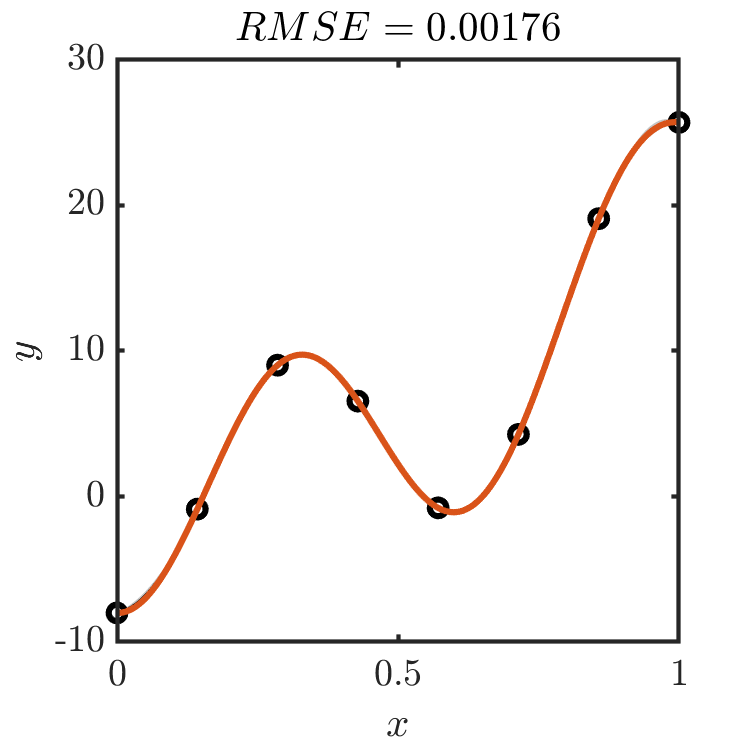
\includegraphics[width=.45\textwidth]{code/image_gen/gp_analytical/images/hf_8.png} }
    \end{subfigure}
    \hfill
    \begin{subfigure}[\label{subfig:gpr_uncertain} With uncertain inputs.]{
        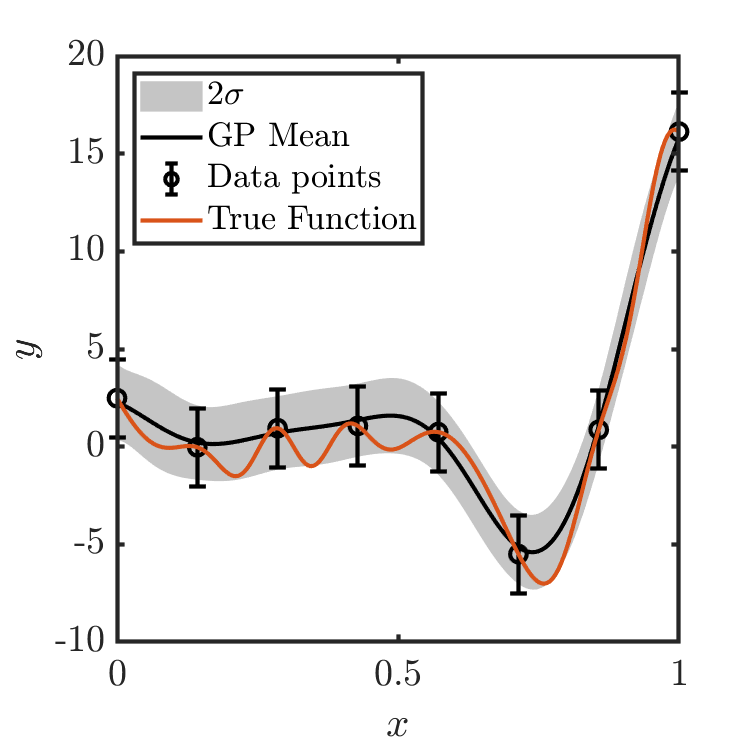
\includegraphics[width=.45\textwidth]{code/image_gen/gp_analytical/images/hf_8_noise.png} 
    }
    \end{subfigure}
    \caption{ GP regression mean and $2\sigma$ error estimates when using deterministic and uncertain input data for an underlying analytic function of interest. \label{fig:gpr_predictions}}
\end{figure}

An important feature of GP regression that is used extensively in this work is the ability to create samples of the GP that are potential representations of the underlying function and take into account the potential errors in the GP. 
A sample mean, $\mu_S(X_*)$ at $X_*$ locations is generated as
\begin{equation} \label{equ:gp_sampling}
    \mu_S(X_*) = \mu(X_*) + \sigma^2(X_*,X_*) U,
\end{equation}
where $U$ is a $n_* \times 1$ vector of random variables drawn from a standard normal distribution $\mathcal{N}(0,1)$.
Figure \ref{fig:gpr_predictions_sample} show samples drawn from the two GP regressions performed on \ref{equ:hf_function} using deterministic and uncertain data. 
Each colored line is a separate sample and represents a potential candidate for the underlying function that is being estimated, based on the limited data that is provided. 

\begin{figure}
    \centering
    \begin{subfigure}[\label{subfig:gpr_deterministic_sample} With deterministic inputs.] {
        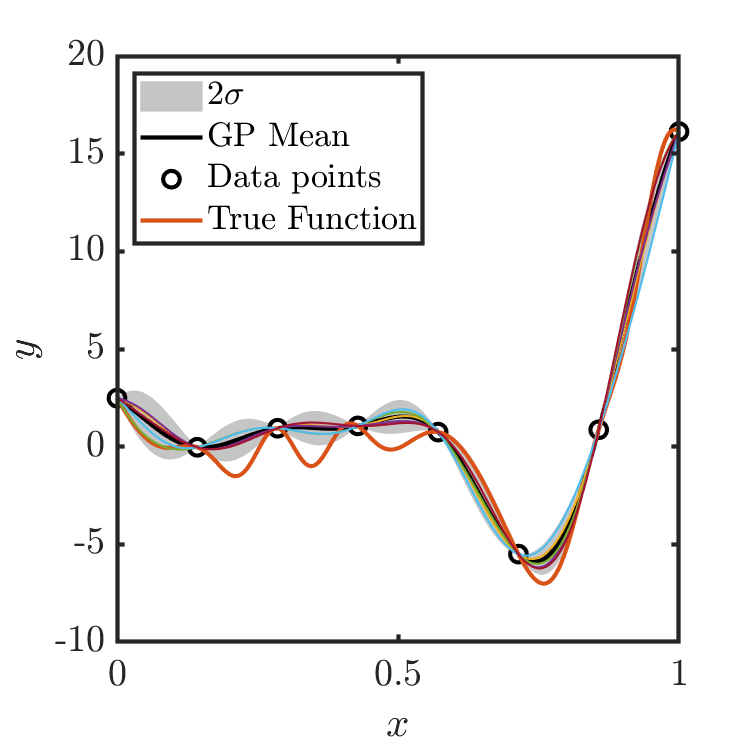
\includegraphics[width=.45\textwidth]{code/image_gen/gp_analytical/images/hf_8_samples.png} }
    \end{subfigure}
    \hfill
    \begin{subfigure}[\label{subfig:gpr_uncertain_sample} With uncertain inputs.]{
        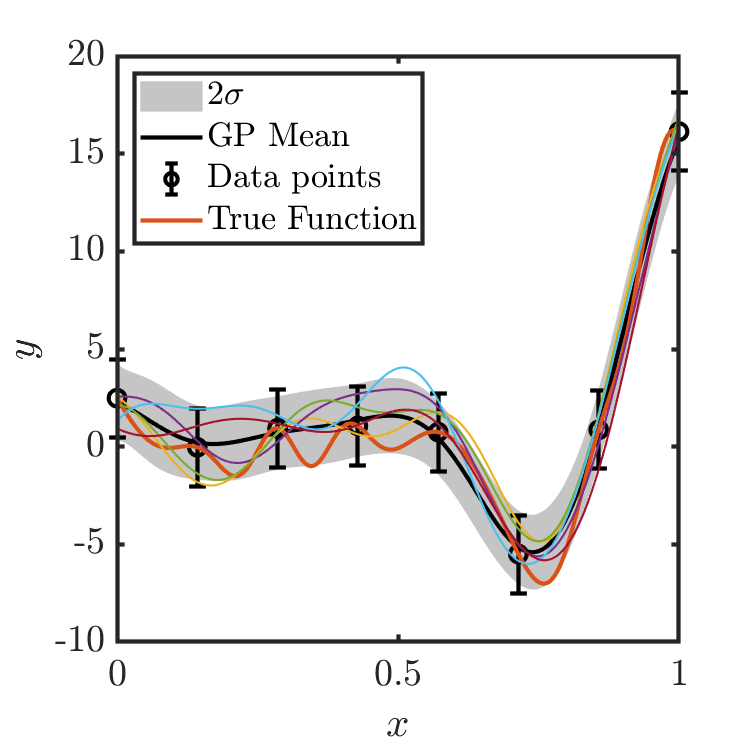
\includegraphics[width=.45\textwidth]{code/image_gen/gp_analytical/images/hf_8_noise_samples.png} 
    }
    \end{subfigure}
    \caption{Samples of the surrogate models that are candidate functions given the GP regression on the deterministic and the uncertain data. \label{fig:gpr_predictions_sample}}
\end{figure}

\section{Multi-Fidelity Gaussian Process Regression} \label{sec:mf_modeling}

It is often the case that simulations or experiments of a sufficiently-high fidelity are too expensive to perform over the entire domain of interest for a modeled problem. In many cases, there are lower-fidelity approximations available that can be evaluated quickly to perform parameter studies. The aim of the multi-fidelity GP is to use data from different fidelity levels to create a surrogate model that can best approximate the highest-fidelity function and its uncertainty, while reducing the required number of high-fidelity function evaluations. 

Assume there are $s$ information sources $f_t(\mathbf{x})$, where $t\in\{1,2,...,s\}$, and the function at the highest fidelity level, $f_s(\mathbf{x})$, is being approximated using a Gaussian Processes, $Z_s(\mathbf{x}) \sim \mathcal{N}(\mu_{s}(\mathbf{x}), \sigma_s^2(\mathbf{x}))$. An auto-regressive formulation of the multi-fidelity framework is used. This was first put forward in \cite{kennedy_predicting_2000} and was improved upon by \cite{gratiet_multi-fidelity_nodate} to reduce computational cost and improve predictions. The GP approximation at the $t$ fidelity level is modeled as

\begin{equation}
    Z_t(\mathbf{x}) = \rho_{t-1}(\mathbf{x})Z_{t-1}(\mathbf{x}) + \delta_t(\mathbf{x}),
\end{equation}
\begin{equation}
    \rho_{t-1}(\mathbf{x}) = \mathbf{g}_{t-1}^T(\mathbf{x})\beta_{\rho_{t-1}},
\end{equation}
where $\mathbf{g}_{t-1}(\mathbf{x})$ is a set of $q$ basis functions, similar to $\mathbf{h}(\mathbf{x})$ in the previous section, $\beta_{\rho_{t-1}}$ is the learned regression coefficients, and $\delta_t(\mathbf{x})$ is modeled using a GP. A way to interpret these terms is to consider $\delta_t(\mathbf{x})$ the additive bias and $\rho_{t-1}(\mathbf{x})$ the multiplicative bias between fidelity levels $t$ and $t-1$. To account for the different fidelity levels and their corresponding data, the subscript $t$ is added to the notation introduced in Section \ref{sec:gpr}. For example, $X_t$ refers to all the input data at level $t$. Additionally, the term $\Sigma_t = \text{diag}(\sigma^2_{i,t})$ is introduced, which refers to the noise in the outputs $\mathbf{y_t}$. 

In Appendix B of \cite{gratiet_multi-fidelity_nodate}, Gratiet presents the predictive equations for the case when the design sets are not nested ($\mathcal{D}_t \notin \mathcal{D}_{t-1}$) and the data has no process noise, such that $\Sigma_t$ is a null matrix. This work extends those equations to include process noise $\Sigma_t \neq \emptyset$, which produces the following representations for the mean and covariance equations for fidelity level $t \neq 1$ as

\begin{equation}\label{equ:mu_Zt}
\begin{split}
    \mu_{t}(X_*) = & ~ \rho_{t-1} \left ( X_* \right ) \mu_{t-1} \left (X_* \right ) + H_*^T\beta_t \\
    & + \left [ \left ( \rho_{t-1} \left (X_* \right ) \rho_{t-1} \left (X_t \right )^T \right ) \odot \sigma^2_{t-1} \left(X_*,X_t \right) + K_{t} \left(X_*,X_t \right)\right] \\ 
    & \times \left [ \left ( \rho_{t-1} \left (X_t \right ) \rho_{t-1} \left (X_t \right )^T \right ) \odot \sigma^2_{t-1} \left(X_t,X_t \right) + V_t \right ]^{-1} \\ 
    & \times \left (\mathbf{y}_t - \rho_{t-1} \left (X_t \right ) \odot \mu_{t-1} \left (X_t \right) - F_t^T \beta_t \right),
\end{split}
\end{equation}
and
\begin{equation}\label{equ:sig_Zt}
\begin{split}
    \sigma^2_{t}(X, \Tilde{X}) = & ~ \left (\rho_{t-1} \left ( X \right ) \rho_{t-1} ( \Tilde{X})^T \right ) \odot \sigma^2_{t-1} (X, \Tilde{X}) + K_t(X, \Tilde{X}) - \\
    & \left [ \left ( \rho_{t-1} \left (X \right ) \rho_{t-1} \left (X_t \right )^T \right ) \odot \sigma^2_{t-1} \left(X,X_t \right) + K_{t} \left(X,X_t \right)\right] \\ 
    & \left [ \left ( \rho_{t-1} \left (X_t \right ) \rho_{t-1} \left (X_t \right )^T \right ) \odot \sigma^2_{t-1} \left(X_t,X_t \right) + V_t \right ]^{-1} \\ 
    & \left [ \left ( \rho_{t-1} \left (X_t \right ) \rho_{t-1} ( \Tilde{X} )^T \right ) \odot \sigma^2_{t-1} (X_t, \Tilde{X} ) + K_{t} ( X_t, \Tilde{X} ) \right], 
\end{split}
\end{equation}
where $(X, \Tilde{X})$ are generic input arguments, $V_t = K_{t} \left(X_t,X_t \right) + \Sigma_t $, and $\rho_{t-1} (X) = G_{t-1}(X)^T \beta_{\rho_{t-1}}$. $G_{t-1}(X)$ is a $q \times n$ matrix where each column is a $q$-dimensional result of the basis functions for the corresponding $m$-dimensional row of input samples in $X$, and $\beta_{\rho_{t-1}}$ are learned regression coefficients. For the lowest fidelity level, $t=1$, the regular GP regression equations, Equations (\ref{equ:mu_gpr}, \ref{equ:sig_gpr}) are used. For a set of sample locations $X_*$, the mean predictions at fidelity level $t$ is given by $\mu_t(X_*)$ and the variance in the predictions is given by the diagonal of $\sigma^2_t(X_*,X_*)$. 

To fully define the GP of each fidelity level, the regression coefficients ($\beta_{\rho_{t-1}}$ and $\beta_t$) and the hyperparameters of the kernel functions of each fidelity level need to be learned from the data. The parameter estimation equations from  \cite{gratiet_multi-fidelity_nodate} are extended for noisy observations:

\begin{equation}
    \begin{bmatrix}
    \beta_t & \beta_{\rho_{t-1}}
    \end{bmatrix} = \left [ J_t^T \left ( K_t(X_t,X_t) + \Sigma_t \right )^{-1} J_t \right ]^{-1} \left [ J_t^T \left ( K_t(X_t,X_t) + \Sigma_t \right ) ^{-1} \mathbf{y_t} \right ], 
\end{equation}
with $J_1 = H_1$ and for $t > 1$, $J_t =  \begin{bmatrix} G_{t-1} \odot \left ( \mu_{t-1} \left ( X_t \right )  \mathbf{1}_{q_{t-1}} \right ) & F_t \end{bmatrix}$. $\mathbf{1}_{q_{t-1}} \in \mathbb{R} ^{q_{t-1} \times n_t} $ is a matrix of ones. The hyperparameters of the kernel functions are learned by minimizing the negative marginal log-likelihood of each fidelity level.

\begin{equation}
    \log~p(\mathbf{y}_t|X;\theta) = -\left (\frac{1}{2} \log|V_t| + \frac{1}{2} \alpha^T V_t^{-1} \alpha + \frac{n_t}{2}\log 2\pi \right),
\end{equation}
where $\alpha = \left (\mathbf{y_t} - \rho_{t-1} \beta_{\rho_{t-1}}-F_t\beta_t \right )$.

To show the potential advantage of using multi-fidelity data to estimate a function of interest, the analytic functions defined by Equations \ref{equ:lf_function} and \ref{equ:hf_function} are used as the low-fidelity approximation and the high-fidelity function of interest respectively. 
For this case, the number of high-fidelity data points is restricted to $4$. 
Figure \ref{subfig:sf_gpr} shows the mean and error estimates for a one-fidelity GP trained on just the 4 high-fidelity data points. 
$\sigma_i^{HF} = 0.3$ in this case.
There aren't enough data points for the GP regression to learn all the nuanced trends in the high-fidelity function of interest. 
For Figure \ref{subfig:mf_gpr}, the low-fidelity function (yellow line) is introduced by using 11 equally spaced function evaluations (blue squares). 
The low-fidelity data doesn't have some of the higher-frequency information that is present in the high-fidelity data, but it approximates the general trends fairly well. 
In this case, the low-fidelity data bolsters the scant $4$ high-fidelity data points, and the multi-fidelity GP that combines both sets of data, is able to provide a more accurate representation of the underlying function of interest. 
It is also important to notice the large error estimates in GP prediction. 
More high-fidelity data would be required to reduce the uncertainty in the GP modeling. 

\begin{figure}
    \centering
    \begin{subfigure}[\label{subfig:sf_gpr} Single-fidelity fit.] {
        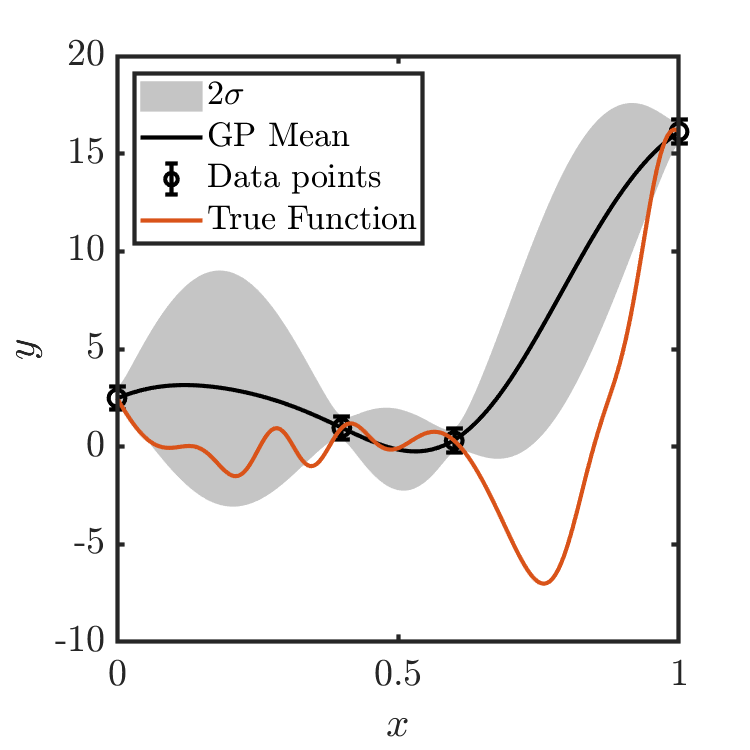
\includegraphics[width=.45\textwidth]{code/image_gen/gp_analytical/images/hf_4_noise.png} }
    \end{subfigure}
    \hfill
    \begin{subfigure}[\label{subfig:mf_gpr} Two-fidelity fit.]{
        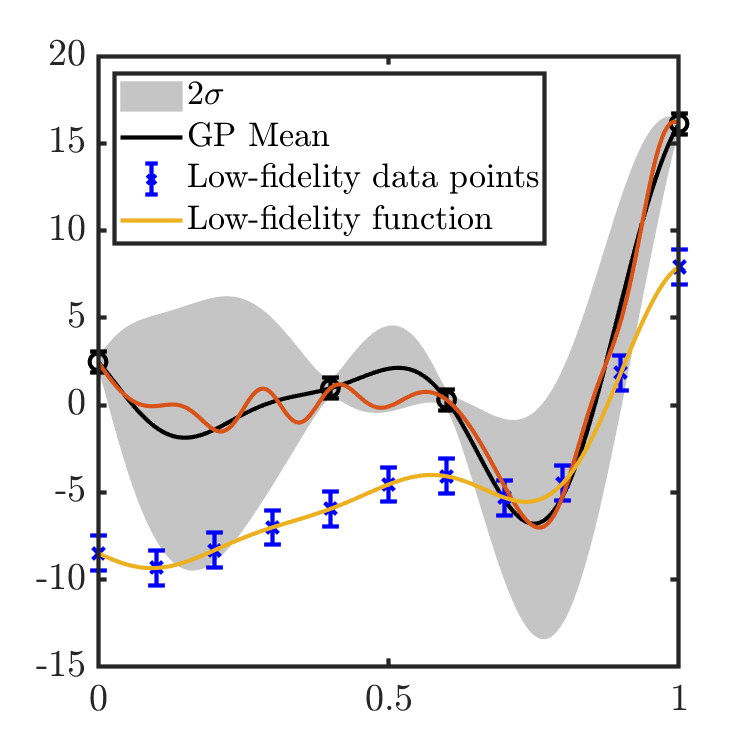
\includegraphics[width=.45\textwidth]{code/image_gen/gp_analytical/images/mf_4_noise.png} 
    }
    \end{subfigure}
    \caption{Comparison of single- and two-fidelity GP regression. \label{fig:mf_vs_sf_analytic}}
\end{figure}

As mentioned earlier in this section, the recursive formulation put forth by Gratiet \cite{le_gratiet_recursive_2014} improves on the work originally done by Kennedy and O'Hagan \cite{kennedy_predicting_2000} by reducing the computational complexity of the training and sampling steps of the multi-fidelity GP.
This is achieved by splitting the dataset into each individual fidelity level instead of agglomerating the data from all levels into one set of equations.
This results in having to invert smaller matrices, which greatly improves the computational cost of the process.
Figure \ref{fig:time_comp} shows the comparative times for the training and sampling steps. Two simple one-dimensional, analytic functions were used to generate the result: 

\begin{equation}
    f_1(x) = 0.5 \left ( 6x - 2\right )^2 \sin{ \left (12x -4 \right )} + 10 \left ( x - 0.5 \right ) -5 ~\text{and}
\end{equation}
\begin{equation}
        f_2(x) = 2f_1(x) - 20x + 20.
\end{equation}
where $f_2(x)$ is the high-fidelity function that is approximated by a lower fidelity function, $f_1(x)$.
In this case, the number of high-fidelity data points ($n_2$) and low-fidelity data points ($n_1$) had a constant ratio: $\frac{n_2}{n_1} = 0.2$. These savings in computational time increase with more fidelity levels and higher-dimensional functions. 

\begin{figure}
    \centering
    \begin{subfigure}[Time taken to train the multi-fidelity GP.] {
        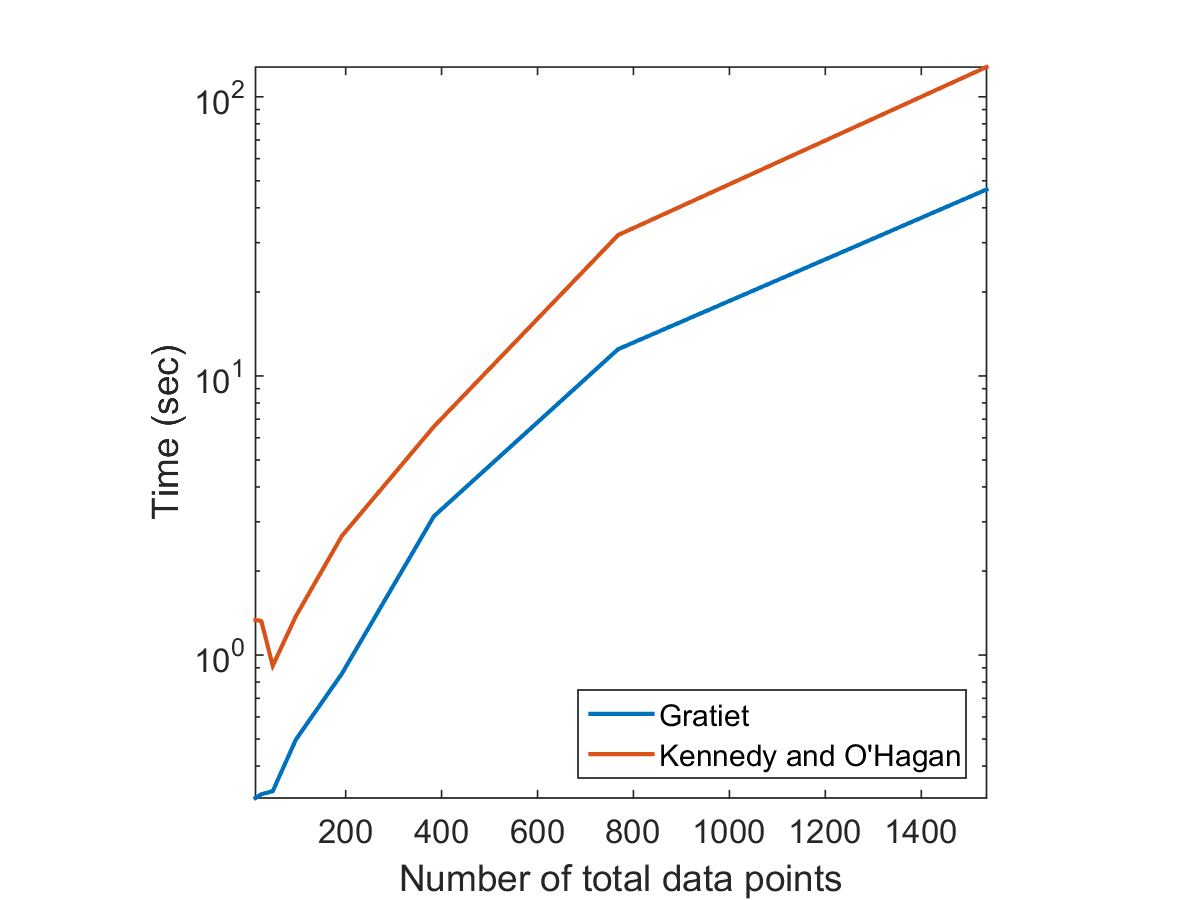
\includegraphics[width=.45\textwidth]{suthesis/images/time_process.png} }
    \end{subfigure}
    \hfill
    \begin{subfigure}[Time taken to sample the multi-fidelity GP.]{
        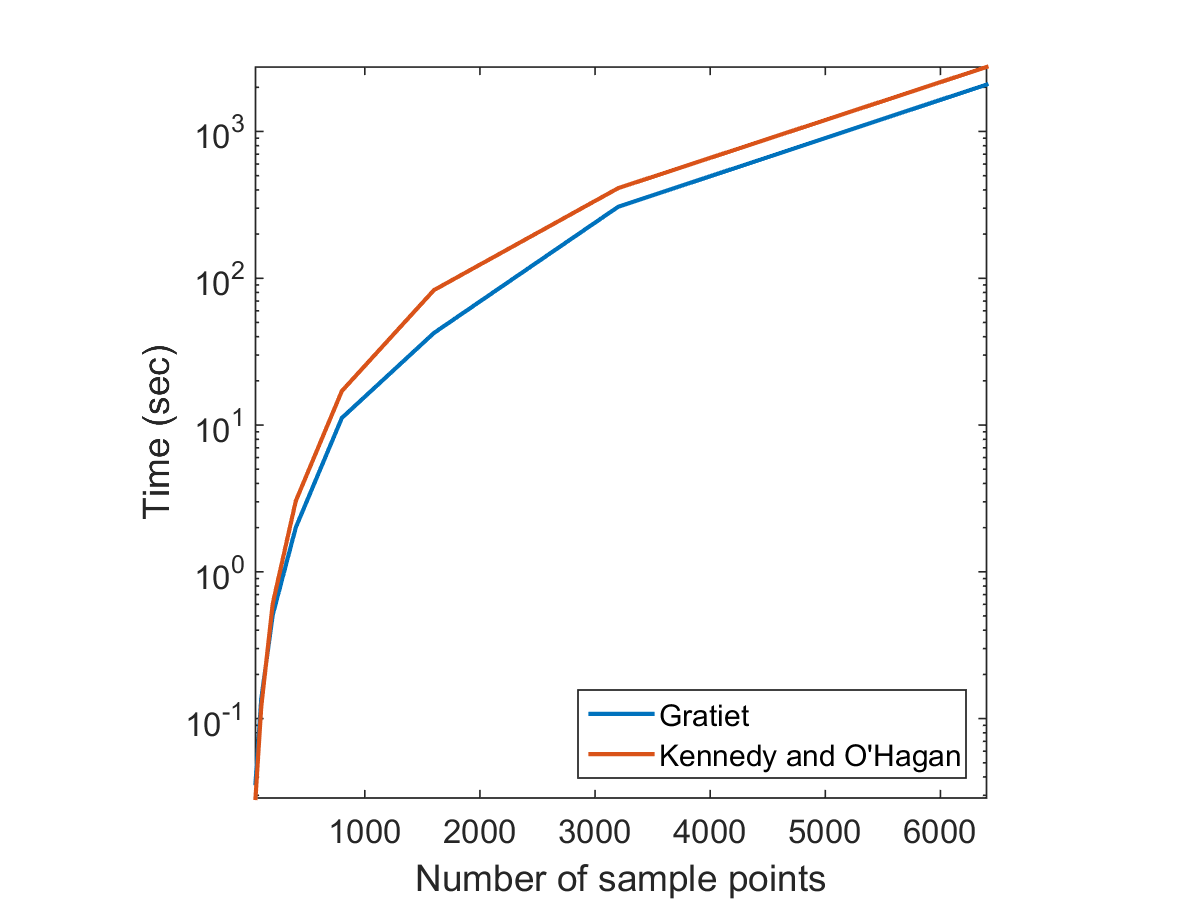
\includegraphics[width=.45\textwidth]{suthesis/images/time_query.png} 
    }
    \end{subfigure}
    \caption{Wall clock time comparison to train and query the multi-fidelity Gaussian Process formulations put forth by Kennedy and O'Hagan \cite{kennedy_predicting_2000}, and Gratiet \cite{gratiet_multi-fidelity_nodate}. \label{fig:time_comp}}
\end{figure}

% \section{Single- vs. Multi-Fidelity Analysis}



\section{Application to NASA CRM} \label{sec:mf_gp_nasa_crm}

To provide more quantitative applications of the RANS UQ methodology, we demonstrate its inclusion in the multi-fidelity GP framework. To showcase the predictive capabilities of the multi-fidelity GP framework, the CFD data is augmented with both low-fidelity simulations, using the Athena Vortex Lattice (AVL) code \cite{drela2008athena}, and high-fidelity experimental data, from the wind tunnel campaigns \cite{rivers_further_2012,rivers_experimental_2010} used in the preceding section. For the vortex-lattice simulations, the uncertainty information is provided by subject matter experts (industry users and academics), while for the experimental data, the uncertainty intervals used are those described in the wind-tunnel campaign reports. 

For the ease of illustration, $C_L$, $C_D$, and $C_m$ are initially considered one-dimensional functions of $\alpha$ ($m = 1$). The methodology described earlier in Section \ref{sec:mf_modeling} is generally applicable to functions of many variables. Aerodynamic databases are often multi-dimensional functions, often with a maximum of 5 input variables (angle of attack, side-slip angle, Mach number, altitude, and dynamic pressure). Multi-dimensional, multi-fidelity databases are explored towards the end of this section. 

The results of the multi-fidelity modeling with one input variable ($\alpha$) are presented in Figures \ref{fig:cl_alpha_mf} -- \ref{fig:cm_alpha_mf}. For each figure, the solid black line represents the mean predicted by the GP and the grey area represents the $\pm 2\sigma$ interval as predicted by the GP. The left column of figures shows purely the AVL data and a single-fidelity GP fit on that data. In the middle we introduce the SU2 RANS CFD data with uncertainty bounds informed by the RANS UQ methodology, and show the two-fidelity GP fit. On the right we introduce a limited set of wind tunnel data points to inform the highest fidelity, and show the resulting three-fidelity fit. For each QoI the build-up of the database is shown, and the distribution of data points across fidelity levels is shown in Table \ref{table:data_points}.

\begin{table}
\centering
    \captionsetup{justification=centering}
    \caption{Number of data points of each fidelity that are used to create Figures \ref{fig:cl_alpha_mf}-\ref{fig:cm_alpha_mf}.} 
    \begin{tabular}{|c|c|}
        \hline
        Data Source & Data Points \\ \hline \hline
        Low Fidelity (AVL) & 23 \\ \hline
        Medium Fidelity (CFD) & 11 \\ \hline 
        High Fidelity (Wind Tunnel) & 5 \\ \hline 
    \end{tabular}
    \label{table:data_points}
\end{table}

In the three-fidelity fits of Figures \ref{fig:cl_alpha_mf}(c) -- \ref{fig:cm_alpha_mf}(c) the wind tunnel data points are evenly spread across the domain of interest, $-2^\circ \leq \alpha \leq 12^\circ$. These data points also have uncertainties associated with them, but these are very small and cannot be seen on this scale in the figures. For the second and third column of figures, the mean and standard deviation predictions are made by the multi-fidelity GP methodology from Section \ref{sec:mf_modeling}. 

\begin{figure}
    \centering
    \begin{subfigure}[Single fidelity fit.] {
        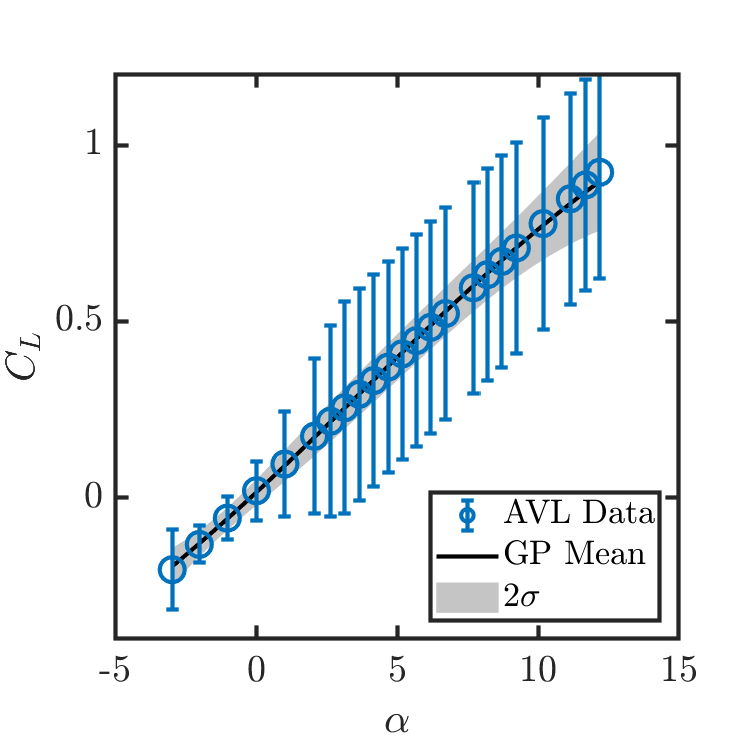
\includegraphics[width=.31\textwidth]{code/image_gen/nasa_crm/images/cl_1f.png} }
    \end{subfigure}
    \hfill
    \begin{subfigure}[Two-fidelity fit.]{
        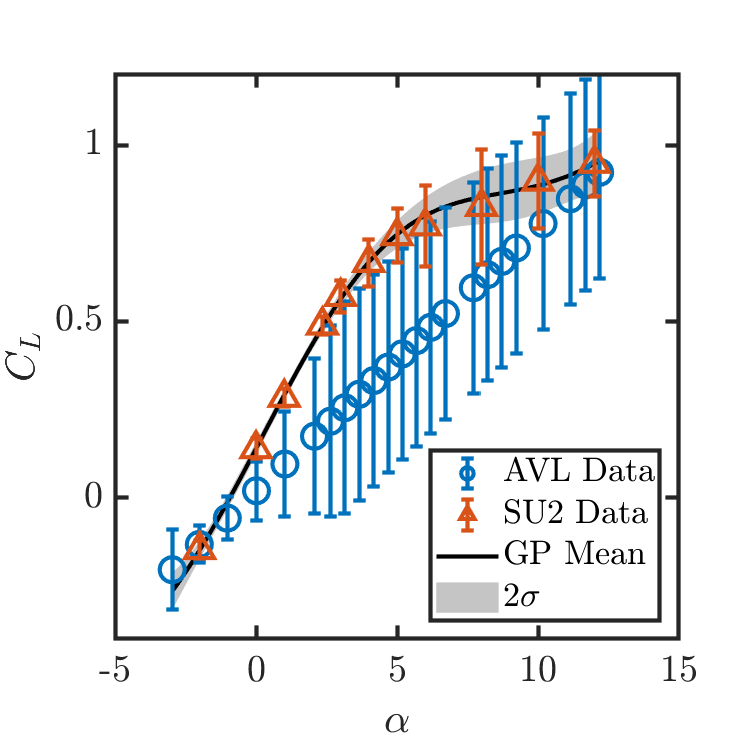
\includegraphics[width=.31\textwidth]{code/image_gen/nasa_crm/images/cl_2f.png} 
    }
    \end{subfigure}
    \hfill
    \begin{subfigure}[Three-fidelity fit.]{
        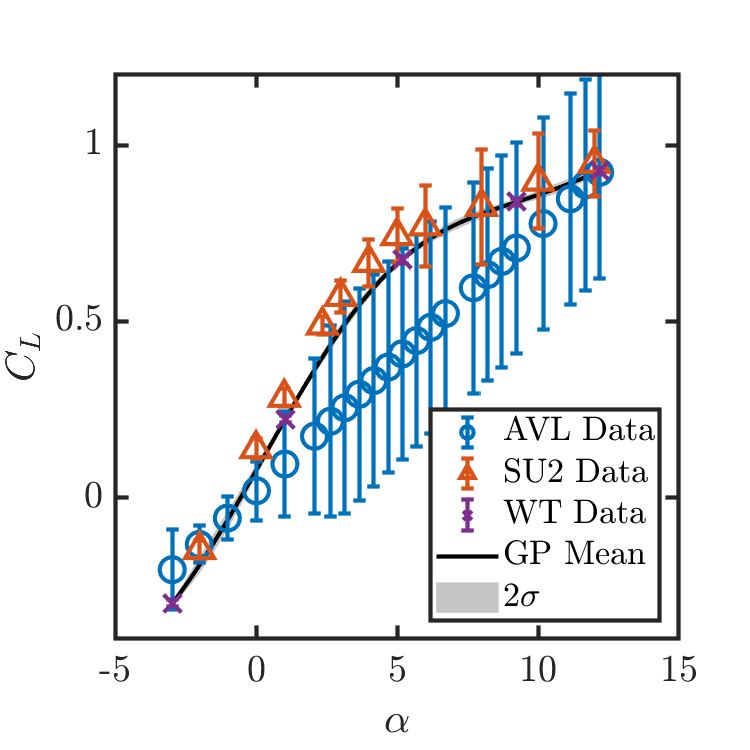
\includegraphics[width=.31\textwidth]{code/image_gen/nasa_crm/images/cl_3f.png} 
    }
    \end{subfigure}
    \caption{$C_L$ vs $\alpha$ for the NASA CRM, using data from multiple sources of varying fidelity.\label{fig:cl_alpha_mf}}
    \hfill
    \centering
    \begin{subfigure}[Single fidelity fit.] {
        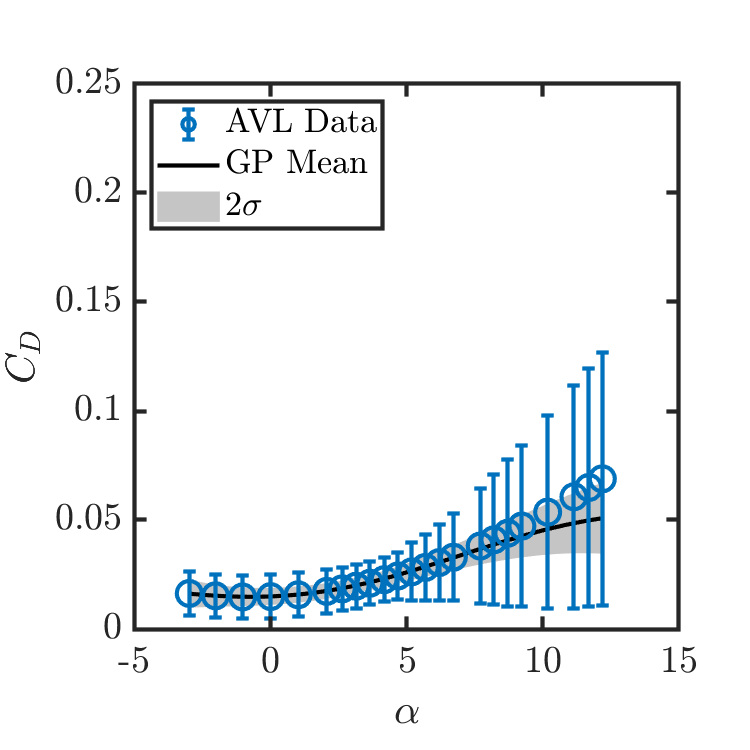
\includegraphics[width=.31\textwidth]{code/image_gen/nasa_crm/images/cd_1f.png} }
    \end{subfigure}
    \hfill
    \begin{subfigure}[Two-fidelity fit.]{
        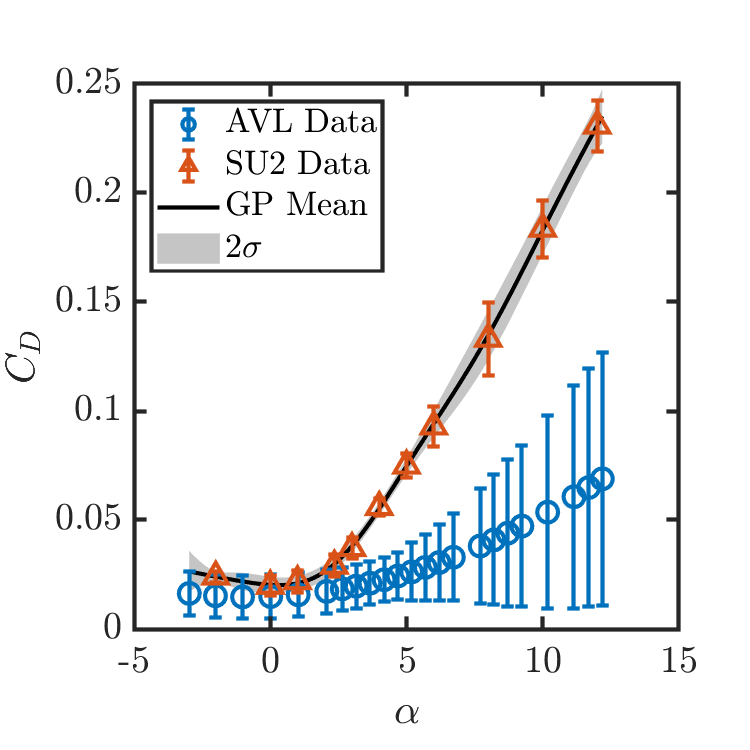
\includegraphics[width=.31\textwidth]{code/image_gen/nasa_crm/images/cd_2f.png} 
    }
    \end{subfigure}
    \hfill
    \begin{subfigure}[Three-fidelity fit.]{
        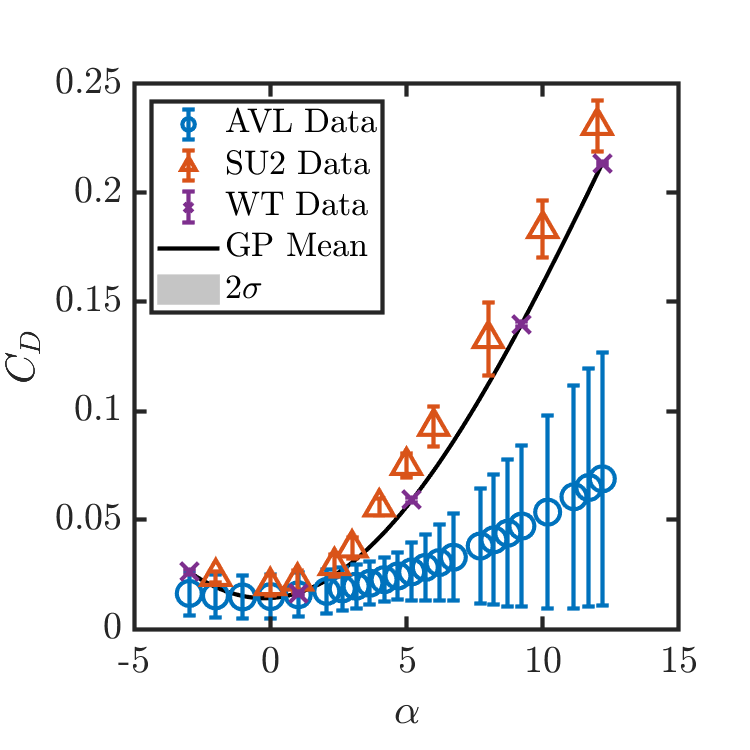
\includegraphics[width=.31\textwidth]{code/image_gen/nasa_crm/images/cd_3f.png} 
    }
    \end{subfigure}
    \caption{$C_D$ vs $\alpha$ for the NASA CRM, using data from multiple sources of varying fidelity.\label{fig:cd_alpha_mf}}
    \hfill
    \centering
    \begin{subfigure}[Single fidelity fit.] {
        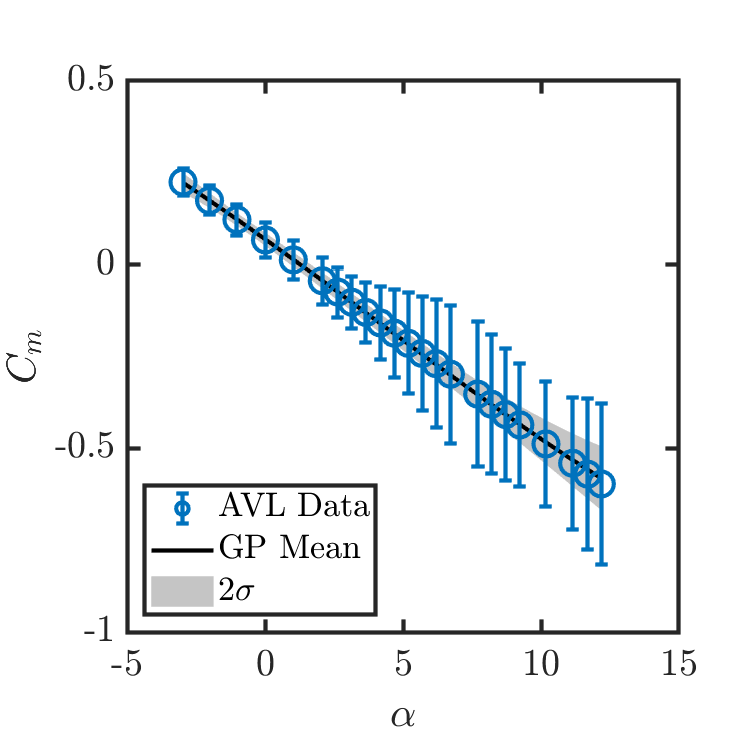
\includegraphics[width=.31\textwidth]{code/image_gen/nasa_crm/images/cm_1f.png} }
    \end{subfigure}
    \hfill
    \begin{subfigure}[Two-fidelity fit.]{
        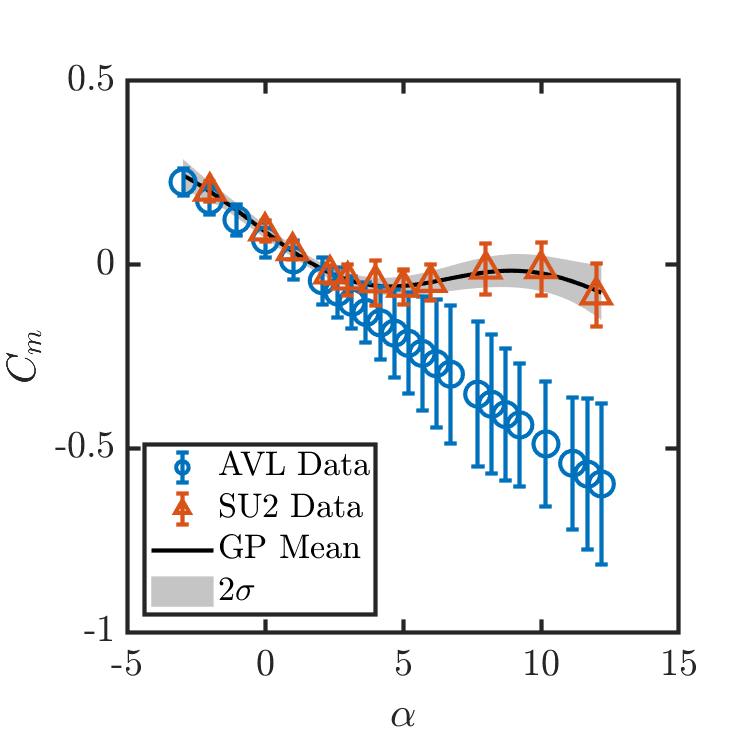
\includegraphics[width=.31\textwidth]{code/image_gen/nasa_crm/images/cm_2f.png} 
    }
    \end{subfigure}
    \hfill
    \begin{subfigure}[Three-fidelity fit.]{
        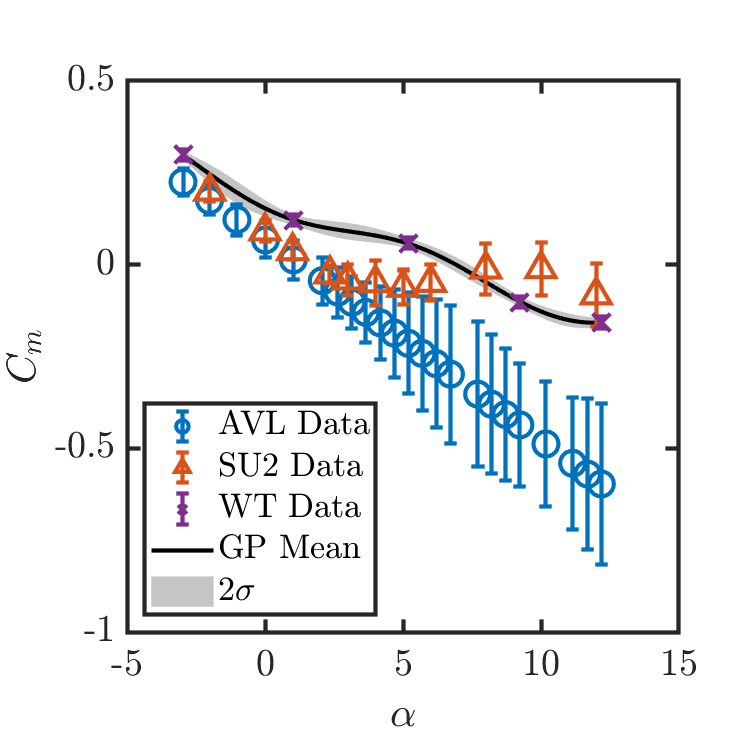
\includegraphics[width=.31\textwidth]{code/image_gen/nasa_crm/images/cm_3f.png} 
    }
    \end{subfigure}
    \caption{$C_m$ vs $\alpha$ for the NASA CRM, using data from multiple sources of varying fidelity.\label{fig:cm_alpha_mf}}
\end{figure}

The multi-fidelity GPs are able to learn the biases between the different fidelity levels and provide predictions that fit very well with the highest fidelity. To show the benefit of using multi-fidelity data vs. using only high-fidelity data points, the root-mean-square error (RMSE) for both cases and for each QoI is presented in Figure \ref{fig:mf_vs_hf}. The error is calculated using the $N$ highest-fidelity data points that aren't used in training the model as:

\begin{equation}\label{equ:rmse}
    RMSE = \sqrt{\frac{\sum_{i=1}^{N}\left ( \mu_{s,i} - y_{s,i} \right )^2}{N}},
\end{equation}
where $y_{s,i}$ is the $i$-th data point of the highest ($s$) fidelity, and $\mu_{s,i}$ is the highest-fidelity prediction from the GP at the same input conditions.  

Since the QoIs are simple functions of $\alpha$, not many high-fidelity data points are required to accurately capture the functional dependence. The differences between the prediction accuracy for a single- vs. multi-fidelity fit is not significant. Nonetheless, the trends are what would be expected. When high-fidelity data is scarce, the multi-fidelity predictions perform better for all QoIs since the low-fidelity data helps provide general trends that are learned by the multi-fidelity GP. As the number of high-fidelity data points increases, the RMSEs converge since there is enough data for both fits to accurately reproduce the functional dependence. When the domain is very well covered by high-fidelity data, the single-fidelity fits can do marginally better since the low-fidelity data (in the multi-fidelity fits) doesn't provide any useful information and can serve to introduce noise in the predictions.

\begin{figure}
    \centering
    \begin{subfigure}[RMSE for $C_L$ vs. $\alpha$.] {
        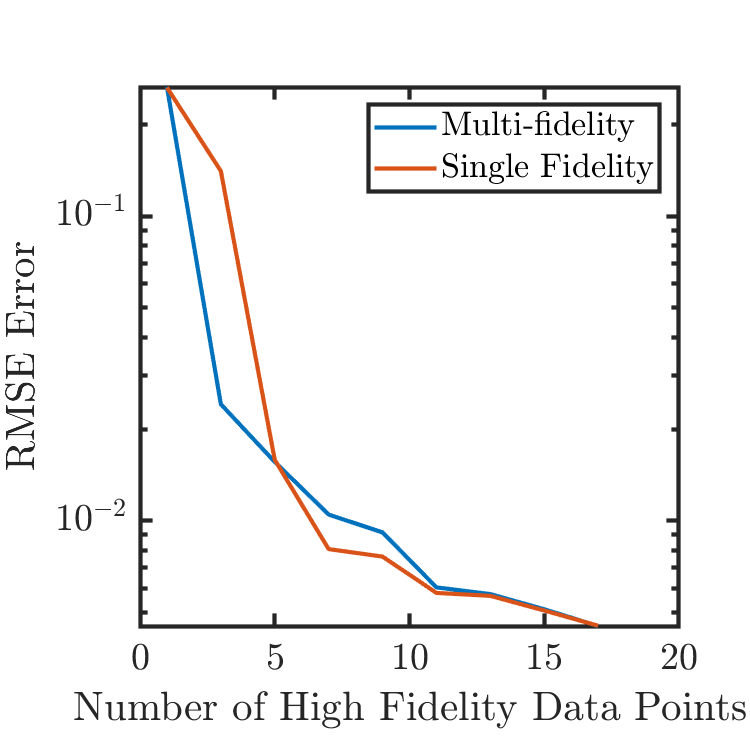
\includegraphics[width=.31\textwidth]{code/image_gen/nasa_crm/images/cl_rsme_comp.png} }
    \end{subfigure}
    \hfill
    \begin{subfigure}[RMSE for $C_D$ vs. $\alpha$.]{
        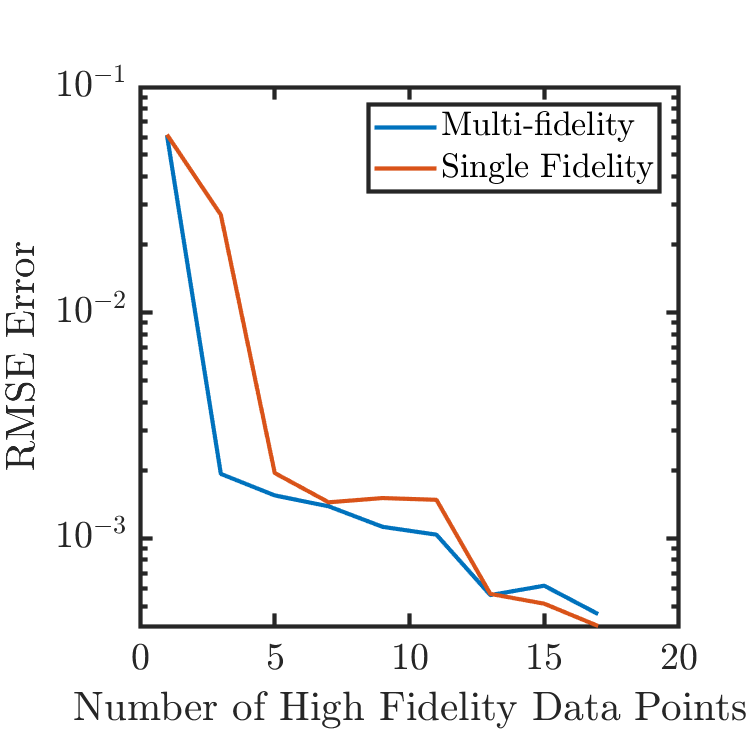
\includegraphics[width=.31\textwidth]{code/image_gen/nasa_crm/images/cd_rsme_comp.png} 
    }
    \end{subfigure}
    \hfill
    \begin{subfigure}[RMSE for $C_m$ vs. $\alpha$.]{
        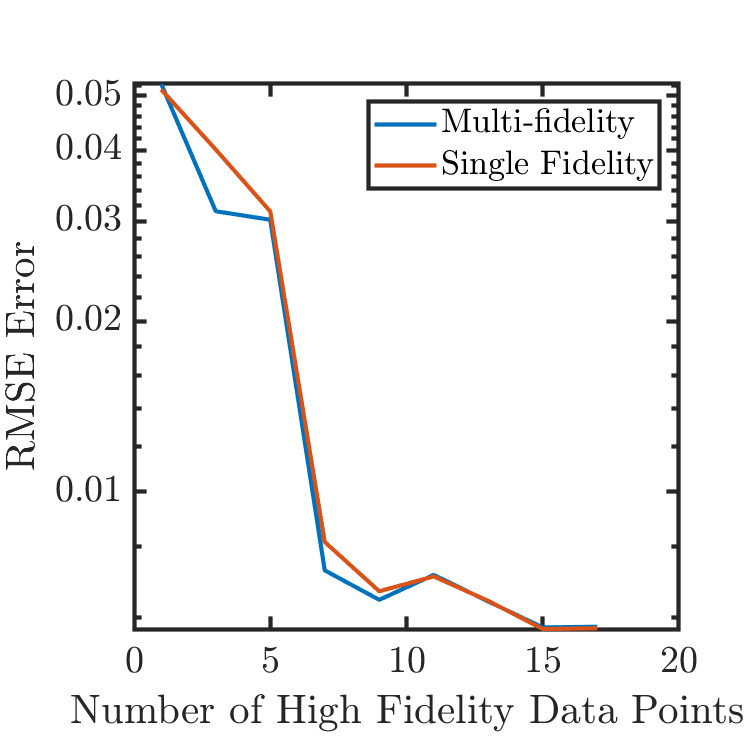
\includegraphics[width=.31\textwidth]{code/image_gen/nasa_crm/images/cm_rsme_comp.png} 
    }
    \end{subfigure}
    \caption{Root Mean Square error when using three-fidelity data vs. using only high-fidelity data points.\label{fig:mf_vs_hf}}
\end{figure}

Another strength of this multi-fidelity GP methodology is apparent when the high-fidelity data is localized to a certain part of the domain. Such a situation might arise if resources are limited and it is not feasible to perform high-fidelity evaluations over the entire domain of interest. It might also be the case that the lower-fidelity simulations are fairly accurate in a certain part of the domain and, consequently, introduce smaller uncertainties in these regions of the domain. For the NASA CRM it is mentioned in Section \ref{sec:crm_rans_uq} that at low angles of attack, where the flow remains attached to the aircraft, RANS CFD simulations are quite successful at predicting performance metrics. This is evidenced by the smaller uncertainty bounds predicted by the RANS UQ methodology in Figure \ref{fig:crm_su2_uq} at $\alpha < 5^\circ$. In this case, an engineer might conclude that highest-fidelity evaluations are not necessary at $\alpha < 5^\circ$ and that sufficient accuracy can be achieved with just the lower-fidelity sources. 

To simulate such a situation, a multi-fidelity GP is created that uses AVL and SU2 data that spans the entire domain of interest, but uses wind tunnel evaluations only at high angles of attack $(\alpha > 5^\circ)$. This is a manufactured situation where we choose to ignore some of the wind tunnel data to illustrate the ability of the multi-fidelity GP framework to perform reliably without high-fidelity information that spans the domain of interest. Figure \ref{fig:mf_partial} presents the predictions made by a three-fidelity GP trained on AVL, SU2, and wind tunnel data (left column), and a single-fidelity GP trained on just the wind tunnel data (middle column). The wind tunnel data used to train the models is restricted to high angles of attack, but the unused wind tunnel data is also included in the plots to discern the quality of the predictions. The right column presents the RMSE of the predictions made by the single- and multi-fidelity GPs when using localized high-fidelity data. The case that is shown in the left and middle columns, is highlighted in this error comparison. From the RMSE comparison, it is clear that having accurate low-fidelity data at low angles of attack informs the GP prediction in that region, and allows it to follow the trend of the physical phenomena more accurately than when only the localized high-fidelity data is used. 

\begin{figure}
    \centering
    \begin{subfigure}[$C_L vs. \alpha$: Three-fidelity fit.] {
        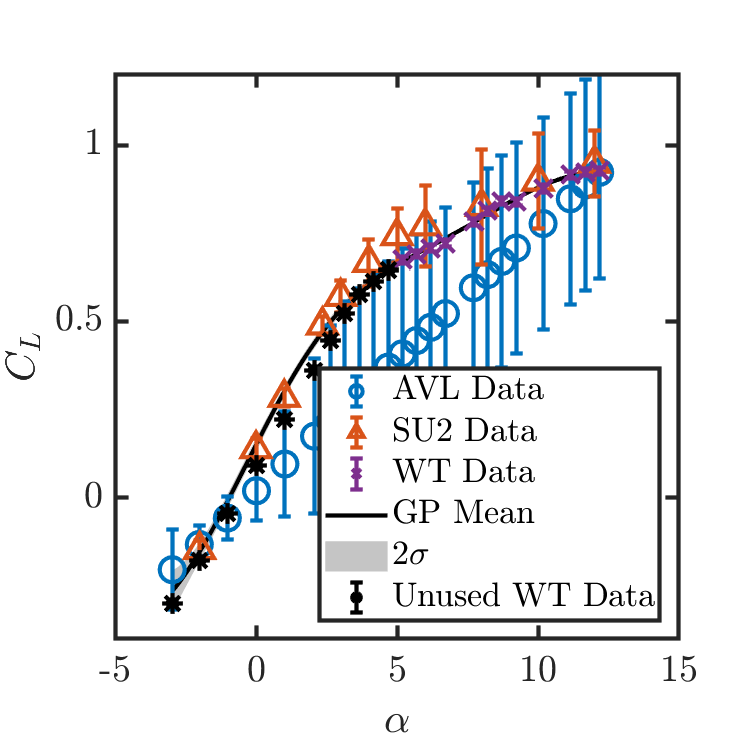
\includegraphics[width=.31\textwidth]{code/image_gen/nasa_crm/images/cl_3f_partial.png} }
    \end{subfigure}
    \begin{subfigure}[$C_L vs. \alpha$: Single fidelity fit.]{
        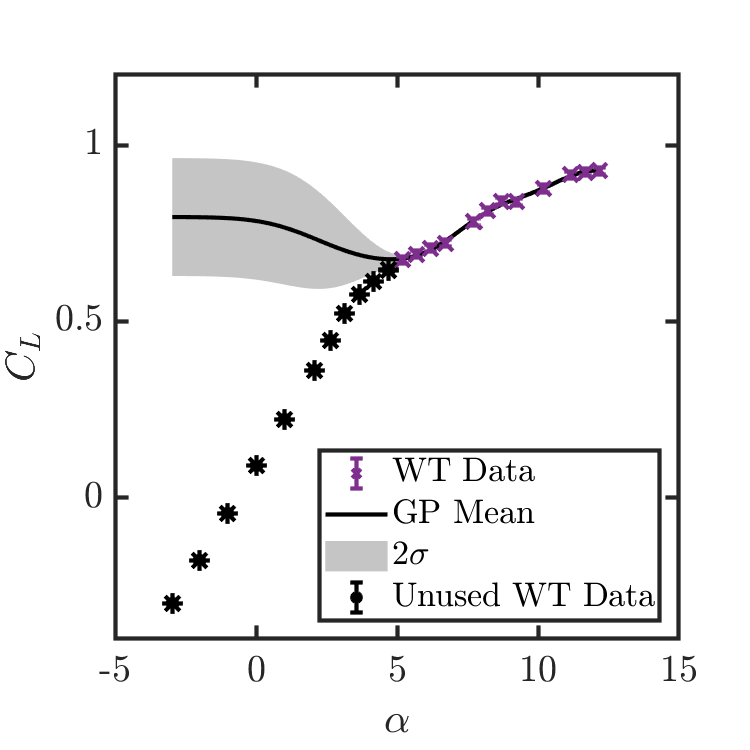
\includegraphics[width=.31\textwidth]{code/image_gen/nasa_crm/images/cl_hf_partial.png} 
    }
    \end{subfigure}
    \hfill
    \begin{subfigure}[$C_L vs. \alpha$: RMSE trends when data is added sequentially from high to low values of $\alpha$.]{
        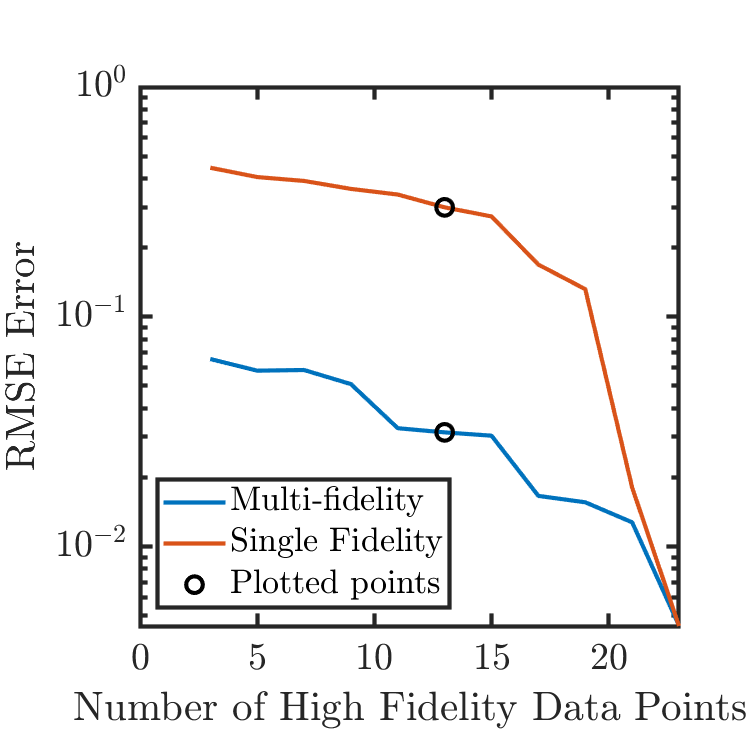
\includegraphics[width=.31\textwidth]{code/image_gen/nasa_crm/images/cl_rsme_local_comp.png} 
    }
    \end{subfigure}

    \begin{subfigure}[$C_D vs. \alpha$: Three-fidelity fit.] {
        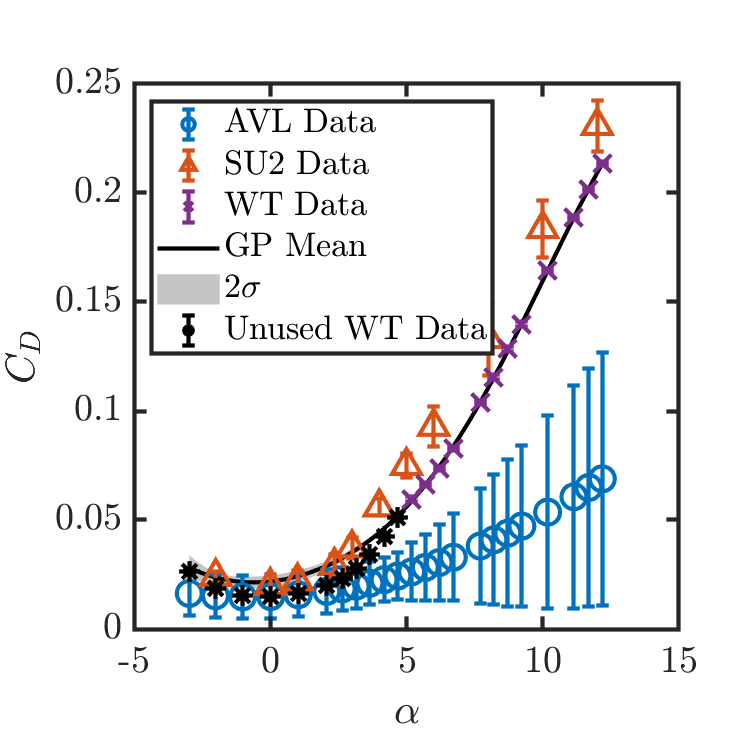
\includegraphics[width=.31\textwidth]{code/image_gen/nasa_crm/images/cd_3f_partial.png} }
    \end{subfigure}
    \begin{subfigure}[$C_D vs. \alpha$: Single fidelity fit.]{
        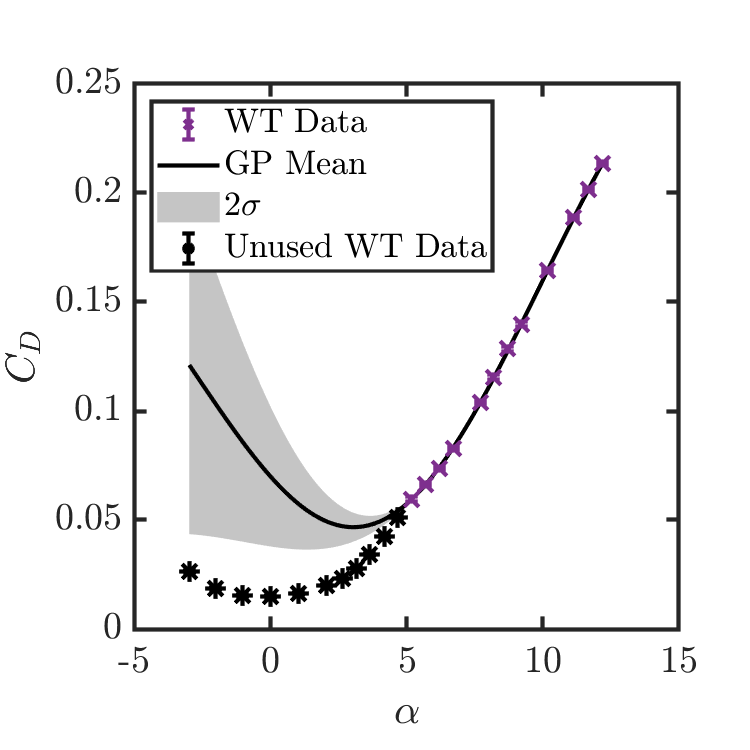
\includegraphics[width=.31\textwidth]{code/image_gen/nasa_crm/images/cd_hf_partial.png} 
    }
    \end{subfigure}
    \hfill
    \begin{subfigure}[$C_D vs. \alpha$: RMSE trends when data is added sequentially from high to low values of $\alpha$.]{
        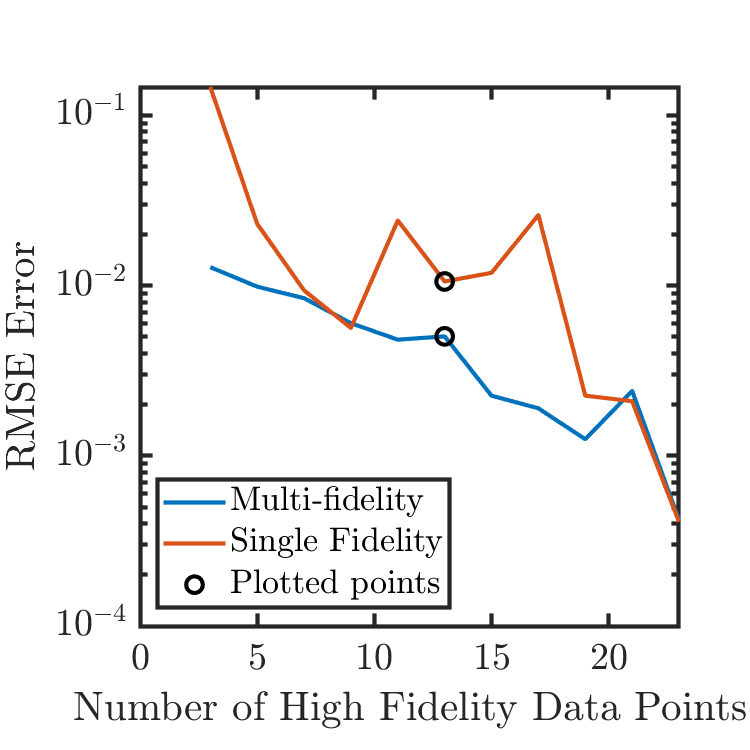
\includegraphics[width=.31\textwidth]{code/image_gen/nasa_crm/images/cd_rsme_local_comp.png} 
    }
    \end{subfigure}

    \begin{subfigure}[$C_m vs. \alpha$: Three-fidelity fit.] {
        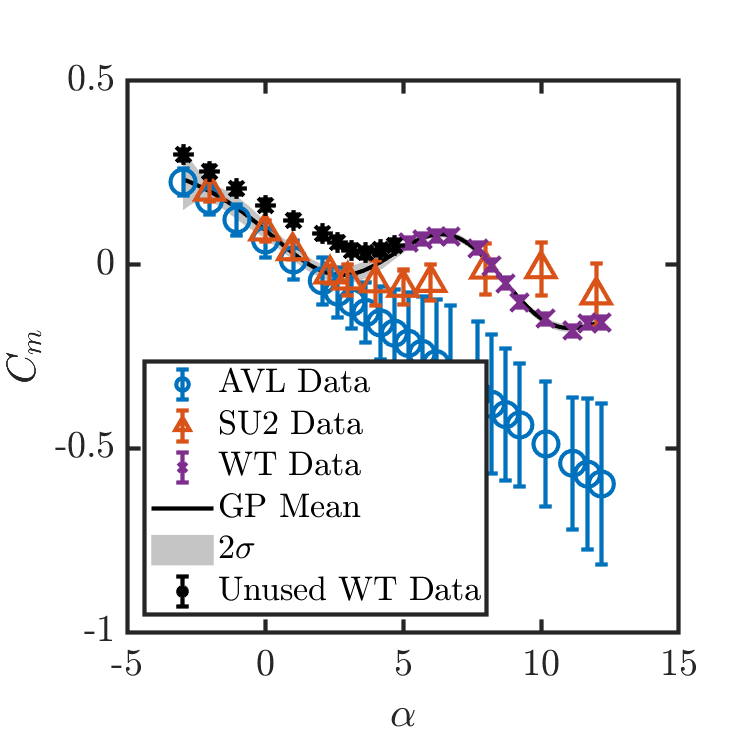
\includegraphics[width=.31\textwidth]{code/image_gen/nasa_crm/images/cm_3f_partial.png} }
    \end{subfigure}
    \begin{subfigure}[$C_m vs. \alpha$: Single fidelity fit.]{
        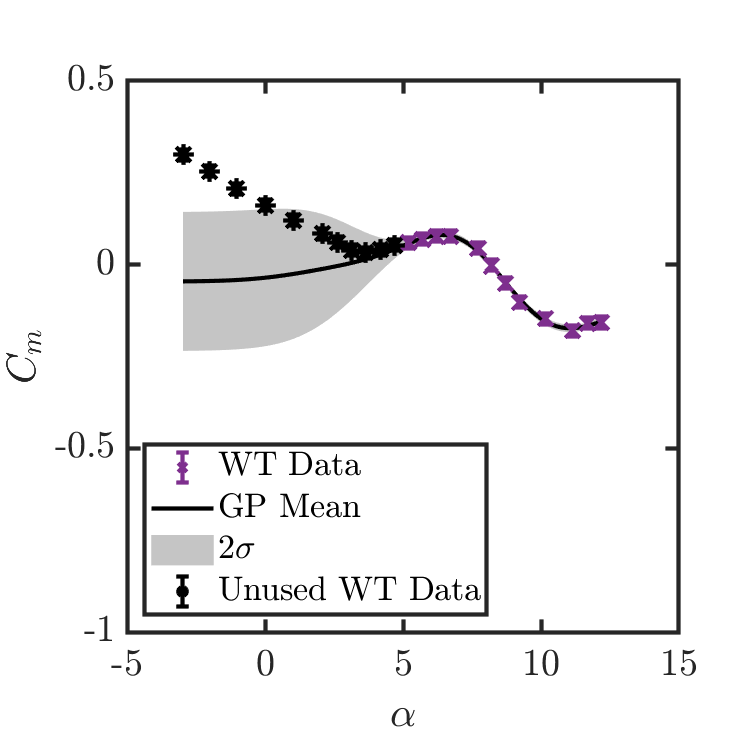
\includegraphics[width=.31\textwidth]{code/image_gen/nasa_crm/images/cm_hf_partial.png} 
    }
    \end{subfigure}
    \hfill
    \begin{subfigure}[$C_m vs. \alpha$: RMSE trends when data is added sequentially from high to low values of $\alpha$.]{
        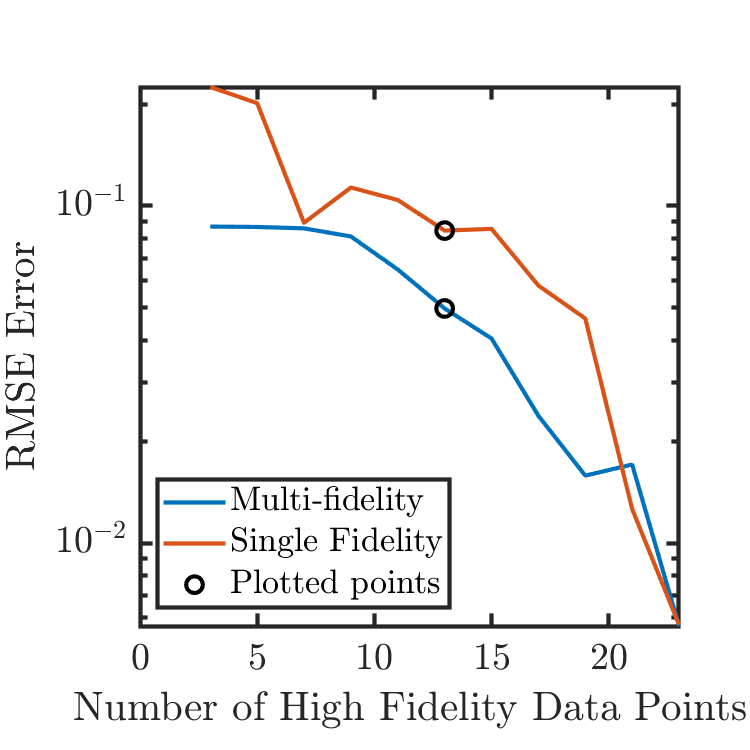
\includegraphics[width=.31\textwidth]{code/image_gen/nasa_crm/images/cm_rsme_local_comp.png} 
    }
    \end{subfigure}
    
    \caption{Showcasing the superior predictive capability of multi-fidelity data fusion when high-fidelity data is localized in the design space. The left column represents the multi-fidelity GP formulation result, while the middle column shows the results for the single-fidelity formulation. The right column shows the RMSE error trends when high-fidelity data is localized. The black circles correspond to the specific case shown in the left and middle columns. \label{fig:mf_partial}}
    
\end{figure}

To explore the performance of the multi-fidelity predictive capability in multiple dimensions, the same aerodynamic coefficients from before ($C_L$, $C_D$, and $C_m$) are considered functions of both $\alpha$ and Mach number. Two sources of information, AVL simulations and wind tunnel data, are used to create two-fidelity, two-dimensional GPs. Visualizing the GP predictions in two dimensions is difficult but the results for $C_L$ are shown in Figure \ref{fig:2d_2f_cl_data}. Figure \ref{fig:cl_2d_2f_points} shows the two-fidelity data sets that are used to train the multi-fidelity GP. Figure \ref{fig:cl_2d_2f_surf} shows the surfaces that represent the mean (as a contoured solid surface), and $2\sigma$ interval estimates (as translucent surfaces sandwiching the mean prediction). The difference between the mean and intervals is hard to discern at that scale. Figure \ref{fig:cl_2d_2f_surf_zoom} focuses in on the high-angle of attack (and low Mach number) area when the uncertainties are larger, to show the different surfaces clearly. To show a one-dimensional representation of the data, a slice spanning the two dimensions is taken (shown in red). The mean and $2\sigma$ intervals along that slice are plotted in Figure \ref{fig:cl_2d_2f_sample}, along with some deterministic samples of the GP (multi-colored lines) that show how they might vary spatially. Again since uncertainties are small, an inset focuses on the high-angle of attack (and low Mach number) area of the domain where the individual samples can be recognized.

\begin{figure}
    \centering
    \begin{subfigure}[AVL and wind tunnel data points.] {
        \label{fig:cl_2d_2f_points}
        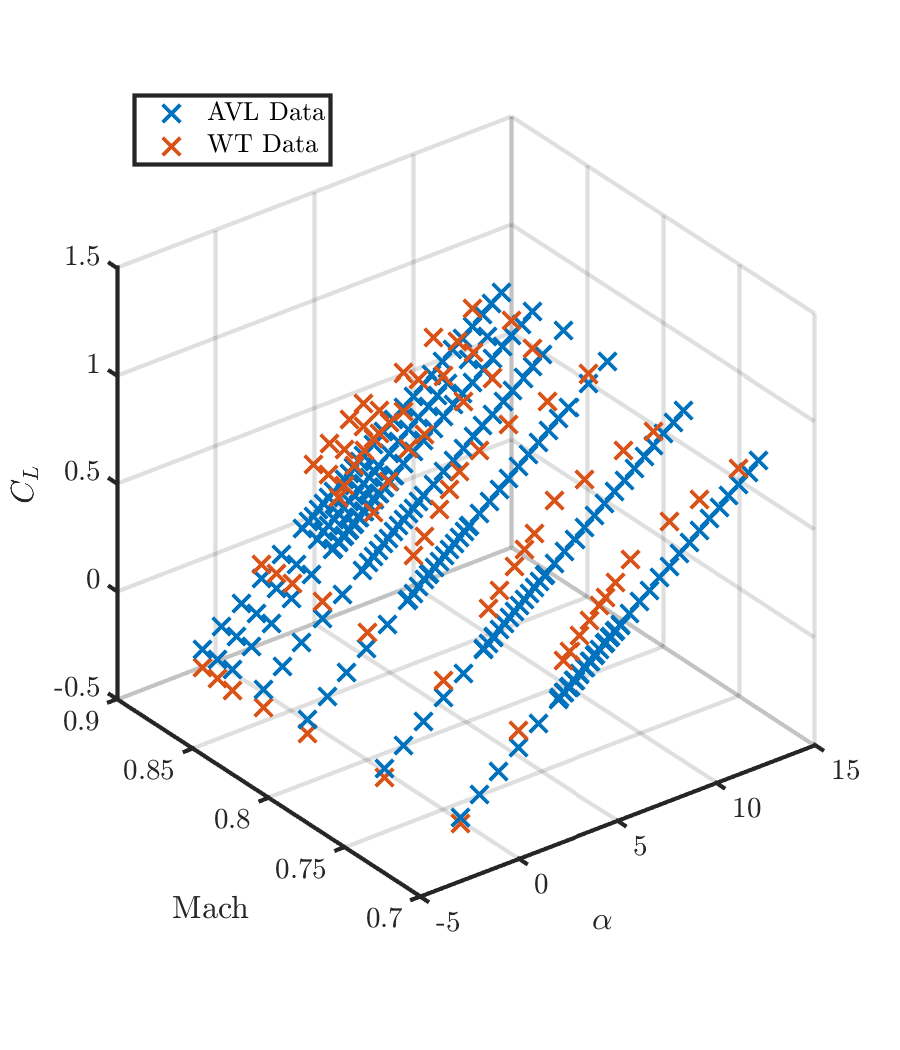
\includegraphics[trim=0 0 0 0, clip, width=.45\textwidth]{code/image_gen/nasa_crm/images/cl_2d_2f_points.png} }
    \end{subfigure}
    \hfill
    \begin{subfigure}[Surfaces representing mean and $2\sigma$ predictions from GP. Red slice shows one-dimensional location for sampling the GP which is shown in \subref{fig:cl_2d_2f_sample}.]{
        \label{fig:cl_2d_2f_surf}
        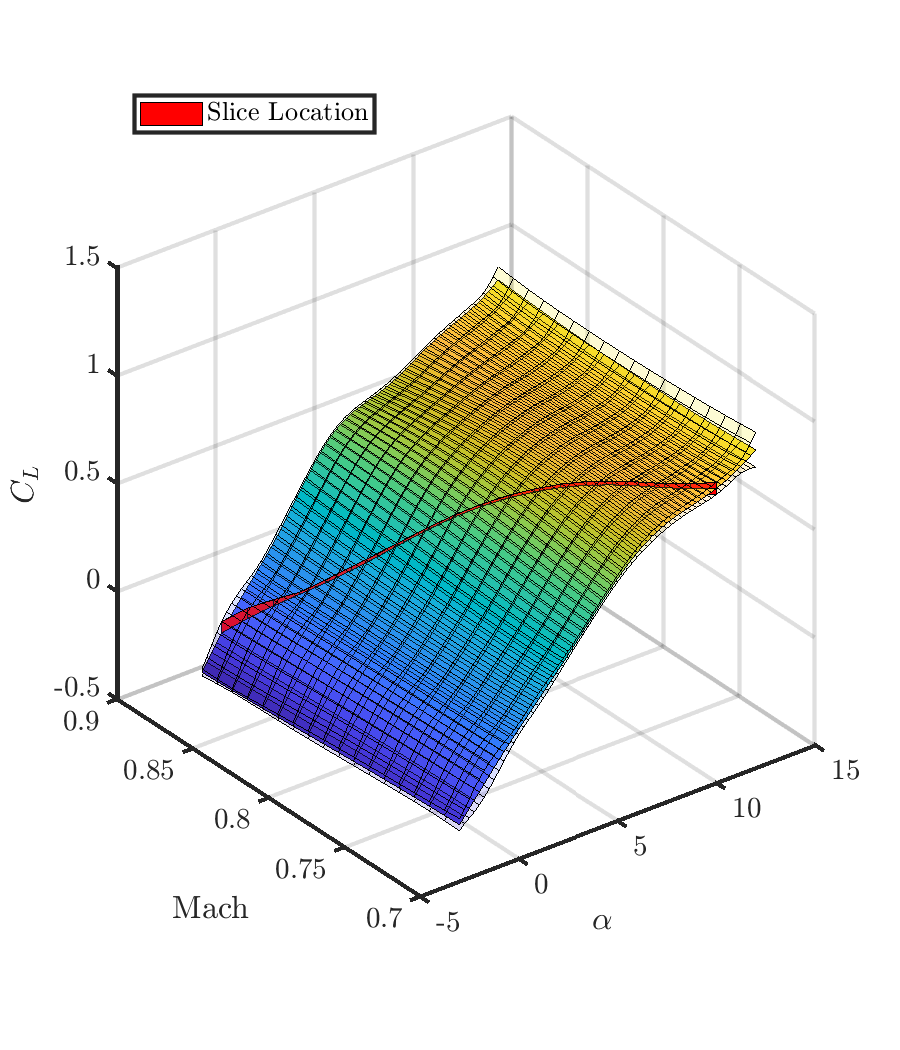
\includegraphics[trim=0 0 0 0, clip, width=.45\textwidth]{code/image_gen/nasa_crm/images/cl_2d_2f_surf.png} 
    }
    \end{subfigure}
    \hfill
    \begin{subfigure}[Zoomed in view of surfaces in \subref{fig:cl_2d_2f_surf} at high angles of attack (and lower Mach number). The mean and $2\sigma$ predictions interval surfaces are more discernible at this scale.]{
        \label{fig:cl_2d_2f_surf_zoom}
        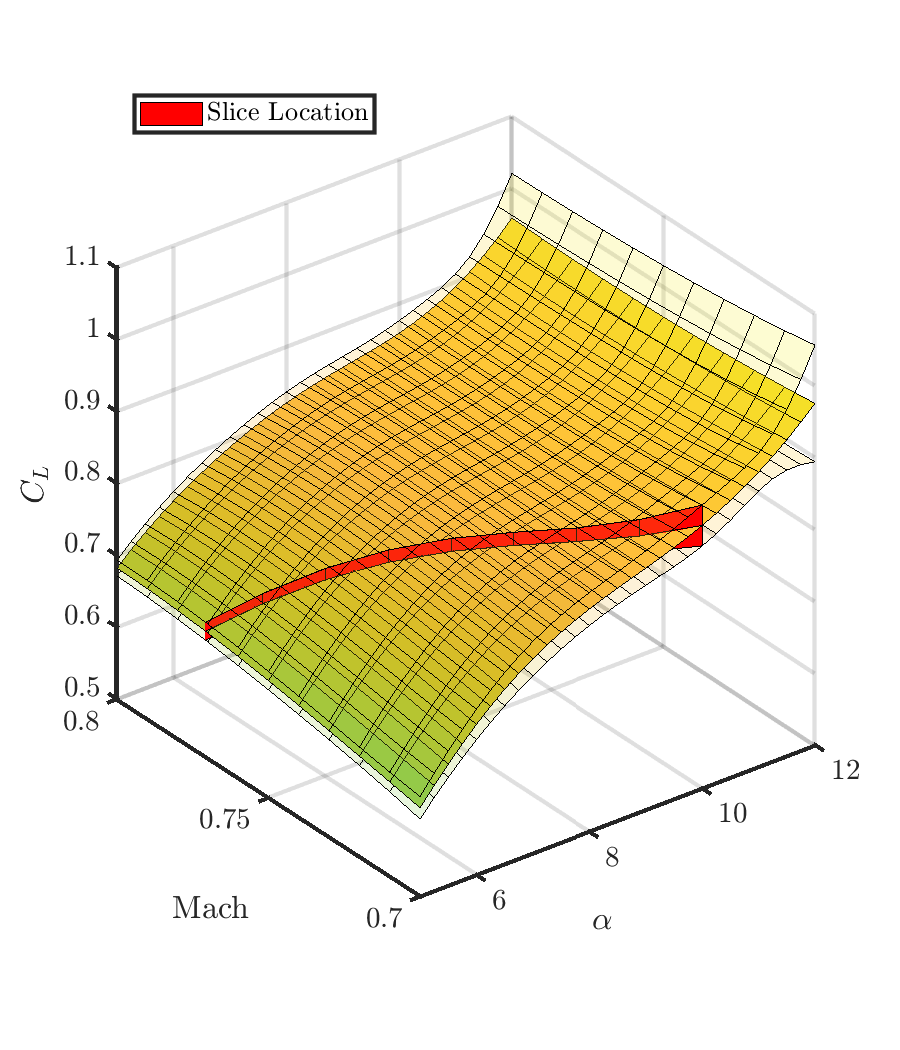
\includegraphics[trim=0 0 0 0, clip, width=.45\textwidth]{code/image_gen/nasa_crm/images/cl_2d_2f_surf_zoom.png} 
    }
    \end{subfigure}
    \hfill
    \begin{subfigure}[One-dimensional representation of mean and $2\sigma$ estimates at slice location shown in \subref{fig:cl_2d_2f_surf}. Multiple samples (colored lines) of the GP are also overlaid to show examples of deterministic sampling. Inset plot focuses in on high angles of attack.]{
        \label{fig:cl_2d_2f_sample}
        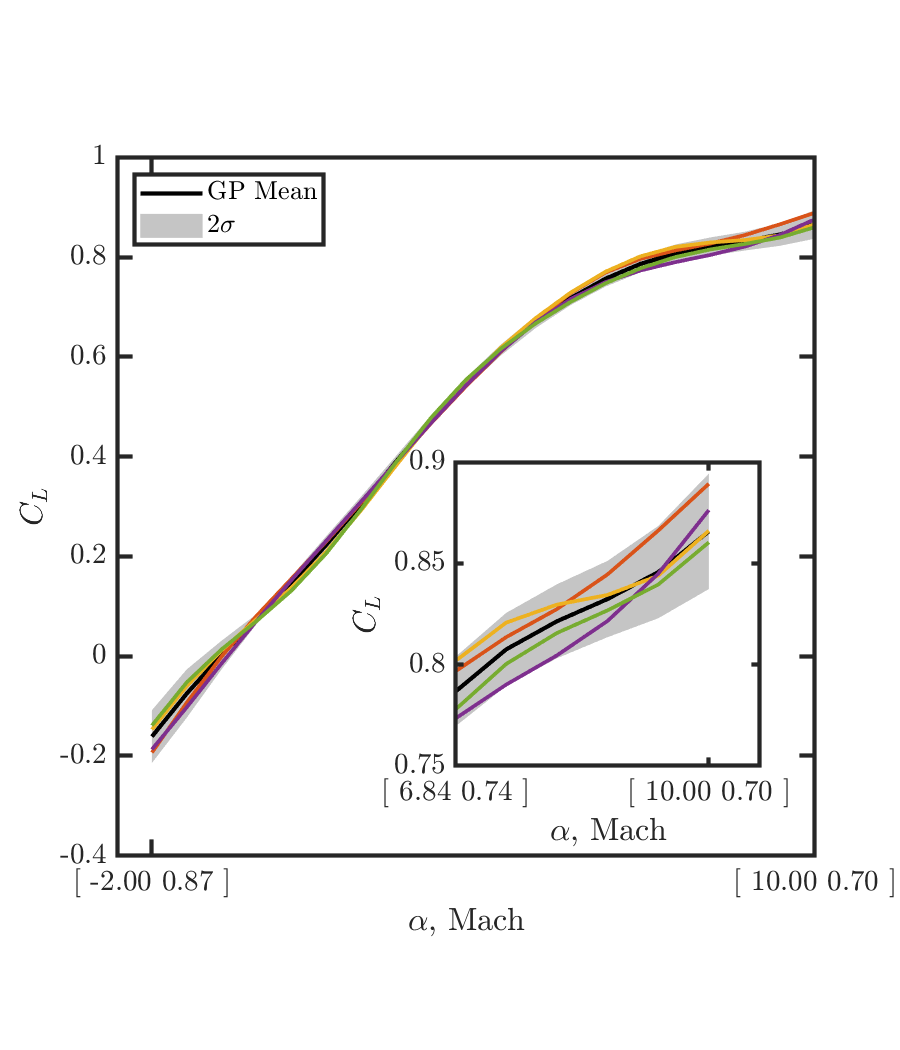
\includegraphics[trim=0 0 0 0, clip, width=.45\textwidth]{code/image_gen/nasa_crm/images/cl_2d_2f_sample.png} 
    }
    \end{subfigure}
    \caption{Two-dimensional representation of $C_L$ as a function of $\alpha$ and Mach number.\label{fig:2d_2f_cl_data}}
\end{figure}

Predictions from the two-fidelity GPs are compared to those made from single-fidelity GPs that use only the wind tunnel data. The change in the root-mean-square-error (Equation \eqref{equ:rmse}) is shown in Fig \ref{fig:2d_mf_vs_hf}. When trying to represent two-dimensional functions, the multi-fidelity fit retains its advantage for longer, with the single-fidelity fit taking $\approx 50$ high-fidelity data points to achieve similar accuracy. If the number of high-fidelity points is increased beyond that, the two fits behave identically. For these results, the high-fidelity data was spread evenly across the domain of interest: $-2^\circ \leq \alpha \leq 12^\circ$ and $0.7 \leq \text{Mach} \leq 0.87$. As the number of input dimensions is increased, more data points would be required to capture the functional trends. Leveraging the multi-fidelity improvement in these high-dimensional spaces would be beneficial in reducing time spent collecting high-fidelity data where a lower-fidelity might suffice.

\begin{figure}
    \centering
    \begin{subfigure}[RMSE for $C_L$.] {
        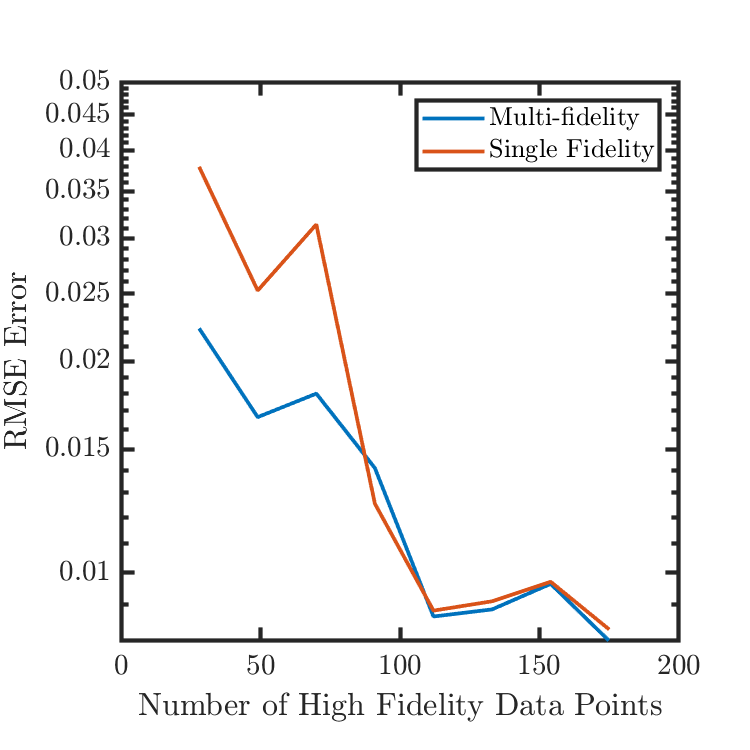
\includegraphics[width=.31\textwidth]{code/image_gen/nasa_crm/images/cl_2d_rsme_lhs_comp.png} }
    \end{subfigure}
    \hfill
    \begin{subfigure}[RMSE for $C_D$.]{
        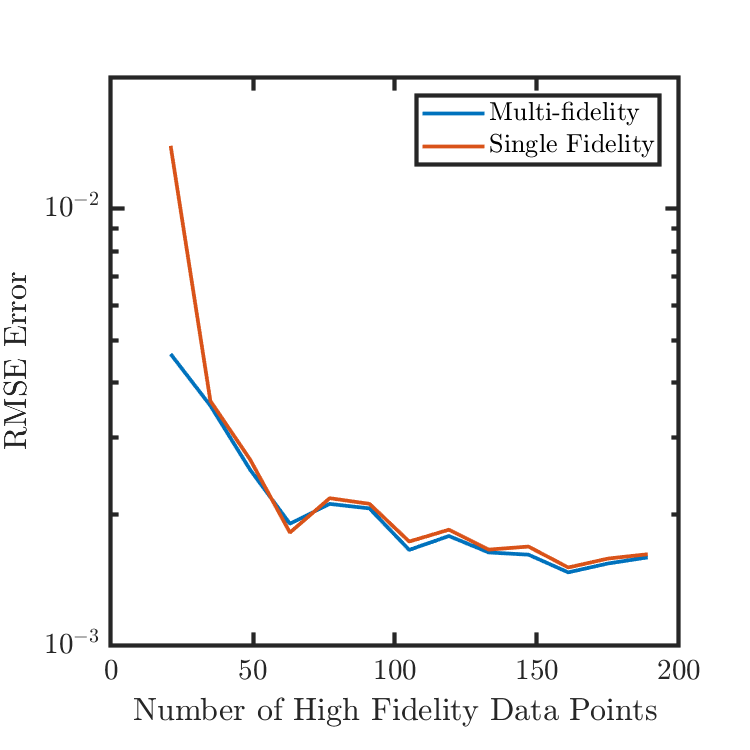
\includegraphics[width=.31\textwidth]{code/image_gen/nasa_crm/images/cd_2d_rsme_lhs_comp.png} 
    }
    \end{subfigure}
    \hfill
    \begin{subfigure}[RMSE for $C_m$.]{
        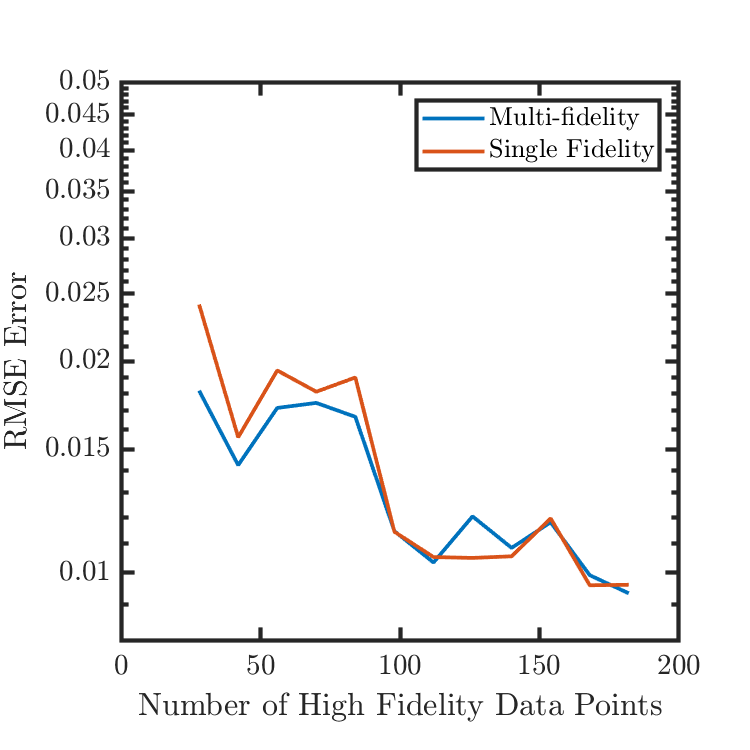
\includegraphics[width=.31\textwidth]{code/image_gen/nasa_crm/images/cm_2d_rsme_lhs_comp.png} 
    }
    \end{subfigure}
    \caption{Root-mean-square-error for two-dimensional functions of Mach and $\alpha$ when using two-fidelity data vs. using only high-fidelity data points.\label{fig:2d_mf_vs_hf}}
\end{figure}



% --------------------------------------
% Aerodynamic Databases
% --------------------------------------
% \chapter{Probabilistic Aerodynamic Databases}

At any point during flight, the air flow over the aircraft exerts certain aerodynamic forces and moments on the airframe. These are a function of the aircraft's geometry, orientation (angle of attack, angle of sideslip etc.), and operating conditions (dynamic pressure, mach number etc.). While designing the aircraft, calculating these forces and moments at various points in its operating envelope helps predict the aircraft's behavior and performance characteristics. Most aerodynamic analyses, be it computational or experimental, are geared towards creating a database that catalogs these values as a function of the aircraft's orientation and operating conditions.

The industry standard is to have a lookup-table that is populated by data from aerodynamic analyses that are performed during the design process. The forces and moments are described as multi-dimensional functions, depending on up to 5 input variables: angle of attack, sideslip angle, mach number, dynamic pressure, and Reynolds number. Discrete analyses in this 5-dimensional domain provide data points that are used interpolate values between analysis locations. These databases are deterministic and have no characterization of the uncertainties present in the analysis techniques, that might affect the data. 

Previous work by Wendorff et al. \cite{wendorff_combining_2016} introduces the concept of probabilistic aerodynamic databases that uses multi-fidelity data and its associated uncertainties in a Gaussian Process regression framework to create a non-deterministic representation of the database. Using a combination of sensitivity and uncertainty analysis, an adaptive sampling technique was developed to find the best location to perform the next analysis to minimize the uncertainty in the objective function at minimum analysis cost. Its application was demonstrated using the NASA CRM configuration performing a longitudinal FAA certification maneuver. 

The current work further matures the probabilistic aerodynamic database concept. Comprehensive, multi-fidelity, multi-dimensional aerodynamics and controls databases are created for a full-configuration generic T-tail transport aircraft that define it's lateral and longitudinal dynamics. Uncertainties in analysis techniques are taken into account, with the CFD uncertainties provided by the eigenspace perturbation methodology introduced in Chapter \ref{chap:rans_uq}.



\section{Aerodynamics and Controls Databases}

An aircraft flies through a multitude of operating conditions during a mission. During takeoff and landing the aircraft flies through dense air in its high-lift configuration at low speeds and high angle of attack. While cruising, the aircraft flies steady and wings-level at high altitude with little controller input. Understanding an aircraft's predicted behavior in all these operating conditions is required for successful certification of the aircraft. 

This work builds large aerodynamics and controls databases by combining multiple sources of information and their associated uncertainties. The generic T-tail transport aircraft is used to demonstrate this capability and consequently all the work shown in this chapter will concern itself with this configuration.

The coefficients that are used to create the aerodynamic database are listed in Table \ref{tab:aero_db}. Force and moment coefficients are two-dimensional functions of angle of attack ($\alpha$) and sideslip angle ($\beta$). Stability derivatives are one-dimensional functions of $\alpha$. 
\begin{table}
    \renewcommand{\arraystretch}{1.2}
    \centering
    \begin{tabular}{ c|c|c|c } 
%  \hline
         Coefficient & Description & Input Variables & Group \\ 
         \hline
         $C_L$ & Coefficient of lift & $\alpha, \beta$  & \multirow{3}{5em}{Force coefficients}\\ 
         $C_D$ & Coefficient of drag & $\alpha, \beta$  \\
         $C_{SF}$ & Coefficient of side force & $\alpha, \beta$  \\ \hline
         $C_l$ & Coefficient of rolling moment & $\alpha, \beta$  & \multirow{3}{5em}{Moment coefficients} \\
         $C_m$ & Coefficient of pitching moment & $\alpha, \beta$  \\
         $C_n$ & Coefficient of yawing moment & $\alpha, \beta$  \\ \hline
         $C_{m_q}$ & Coefficient of pitching moment due to pitch rate & $\alpha$  & \multirow{5}{5em}{Stability derivatives}\\
         $C_{l_p}$ & Coefficient of rolling moment due to roll rate & $\alpha$ \\
         $C_{l_r}$ & Coefficient of rolling moment due to yaw rate & $\alpha$ \\
         $C_{n_p}$ & Coefficient of yawing moment due to roll rate & $\alpha$ \\
         $C_{n_r}$ & Coefficient of yawing moment due to yaw rate & $\alpha$
         \\
        %  \hline
    \end{tabular}
    \caption{List of aerodynamic coefficients that are used to make up the aerodynamic database}
    \label{tab:aero_db}
\end{table}

Similarly, the coefficients used to create the controls database are listed in Table \ref{tab:control_db}. Except for the case with elevator deflections, all coefficients are three-dimensional functions of $\alpha$, $\beta$, and control surface deflection ($\delta_*$). Since flaps change the baseline aerodynamics of the aircraft, its effect on force coefficients is included in the controls database. This is not the case for the other control surfaces, where only their effect on moment coefficients is used. 

\begin{table}
    \renewcommand{\arraystretch}{1.2}
    \centering
    \begin{tabular}{ c|c|c } 
%  \hline
         Control Surface & Coefficients Used & Input Variables \\ 
         \hline
         Ailerons & $C_l, C_m, C_n$ with deflected ailerons & $\alpha, \beta, \delta_a$  \\
         Elevator & $C_l, C_m, C_n$ with deflected elevator & $\alpha, \delta_e$  \\
         Rudder & $C_l, C_m, C_n$ with deflected rudder & $\alpha, \beta, \delta_r$  \\
         Flaps & $C_L, C_D, C_{SF}, C_l, C_m, C_n$ with deflected flaps & $\alpha, \beta, \delta_f$  \\
         Spoilers & $C_l, C_m, C_n$ with deflected spoilers & $\alpha, \beta, \delta_s$  \\
        %  \hline
    \end{tabular}
    \caption{List of controls surface coefficients that are used to make up the controls database}
    \label{tab:control_db}
\end{table}

It is important to note that true control derivatives, such as $C_{l_{\delta_a}}$, aren't calculated. Calculating the derivative using finite differencing is susceptible to numerical issues. Rather the change in the moment coefficient due to the deflected control surface is used. For example: 

\begin{equation}\label{equ:control_derivative}
    C_{l_{\delta_a}}(\alpha,\beta,\delta_a) = C_l(\alpha,\beta,\delta_a) - C_l(\alpha,\beta,\delta_a=0)
\end{equation}

The discrete data for each coefficient, and its associated uncertainty, is used to train a Gaussian process. Individual multi-fidelity Gaussian processes are used to model each coefficient.

\section{Multi-Fidelity Data}

Multiple analysis techniques with varying fidelity levels are used during the aircraft design process to predict performance characteristics. Earlier in the design process, where there is more freedom in design, 

\section{Construction and Sampling}

\section{Databases for the Generic T-tail Transport Aircraft} \label{sec:gtt_dbs}

Thus far, the examples of probabilistic databases have focused on the baseline aerodynamics of the aircraft in question. 
This section will focus on controls databases that define the aircraft's response to a control surface deflection by providing the imparted rotational moments. 
As mentioned in Section \ref{subsec:gtt_cfd_data_gen}, the difficulty in modeling control surface deflections precludes the use of CFD simulation data in building these controls databases. 
Consequently, these databases can be, at most, two-fidelity ones with AVL simulations and wind tunnel experiments as the data sources. 
This section presents several visualizations of the GP regressions.
Single-fidelity GP results using AVL data and WT data in isolation are contrasted with the two-fidelity GP results that use both sets of data to showcase the advantages of using multi-fidelity data.

In the interest of brevity and since the maneuver of interest focuses on the roll-authority of the aircraft, these visualizations will present the roll moment imparted due to aileron deflection ($C_{l_{\delta_a}}$).
This variable is just one of the 18 coefficients (Table \ref{tab:control_db}) that define the aircraft's control behavior, but it is the most pivotal for the maneuver of interest. 

\subsection{Single-fidelity Databases}

Figures \ref{fig:gtt_avl_ctrl_gps} and \ref{fig:gtt_wt_ctrl_gps} present the results of the single-fidelity GP regression performed on AVL data and wind tunnel data, respectively. 
With controls databases, a new input variable defining the control surface deflection angle ($\delta_*$) is used in addition to $\alpha$ and $\beta$ .
This additional variable makes visualizing the results of the 3-dimensional GP in 3D space challenging. 
Both sets of figures show four surfaces or lines in the first three subfigures. 
Each line or surface corresponds to the GP prediction at a particular aileron deflection angle.
For each of the figures, the lines/surfaces are stacked in order of increasing deflection angle, where the angles are $\delta_a \in \{-25^\circ, -10^\circ, 10^\circ, 25^\circ\}$. 
These deflection angles are chosen because the wind tunnel experiments were carried out with these aileron deflection angles. 

\begin{figure}
    \centering
    \begin{subfigure}[\label{subfig:gtt_avl_ctrl_surf}3-Dimensional function in $\alpha$, $\beta$, and $\delta_a$] {
        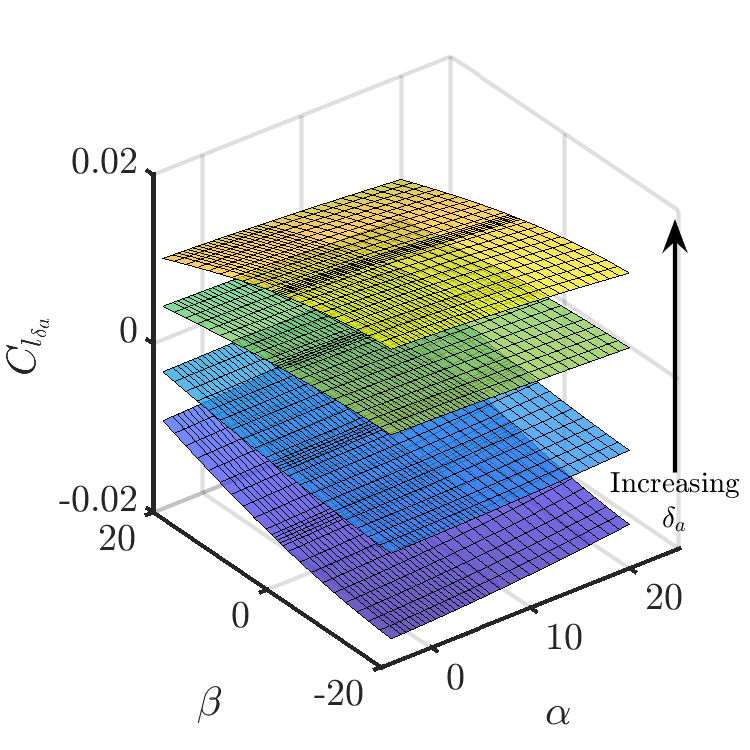
\includegraphics[trim=0 0 0 0, clip, width=.48\textwidth]{code/image_gen/gmatt/1f/avl/images/gps/CRMAIL.png} }
    \end{subfigure}
    \hfill
    \begin{subfigure}[\label{subfig:gtt_avl_ctrl_beta}Variation in $\beta$ at $\alpha=8^\circ$]{
        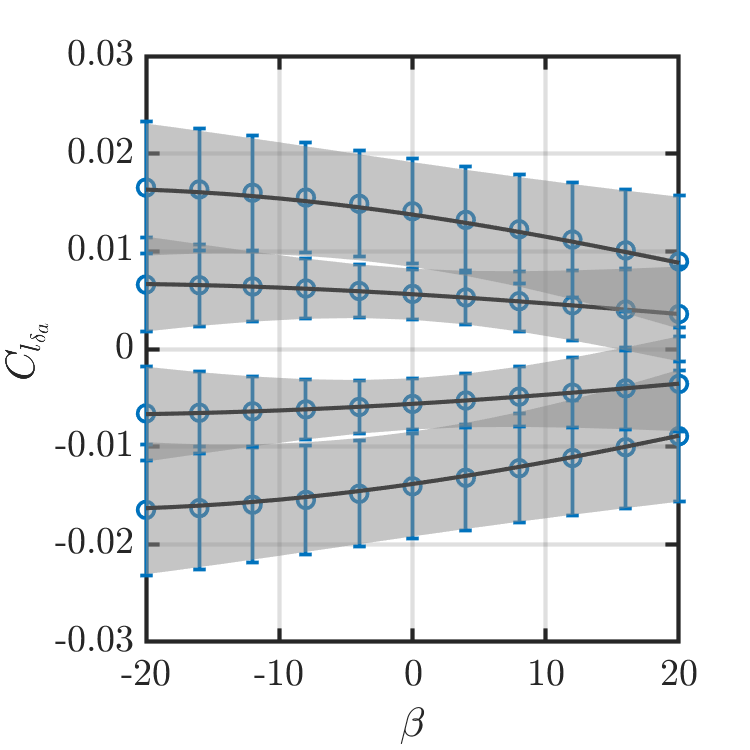
\includegraphics[trim=0 0 0 0, clip, width=.48\textwidth]{code/image_gen/gmatt/1f/avl/images/gps/CRMAIL_alpha=8.png}
    }
    \end{subfigure}
    \hfill
    \begin{subfigure}[\label{subfig:gtt_avl_ctrl_alpha}Variation in $\alpha$ at $\beta=4^\circ$]{
        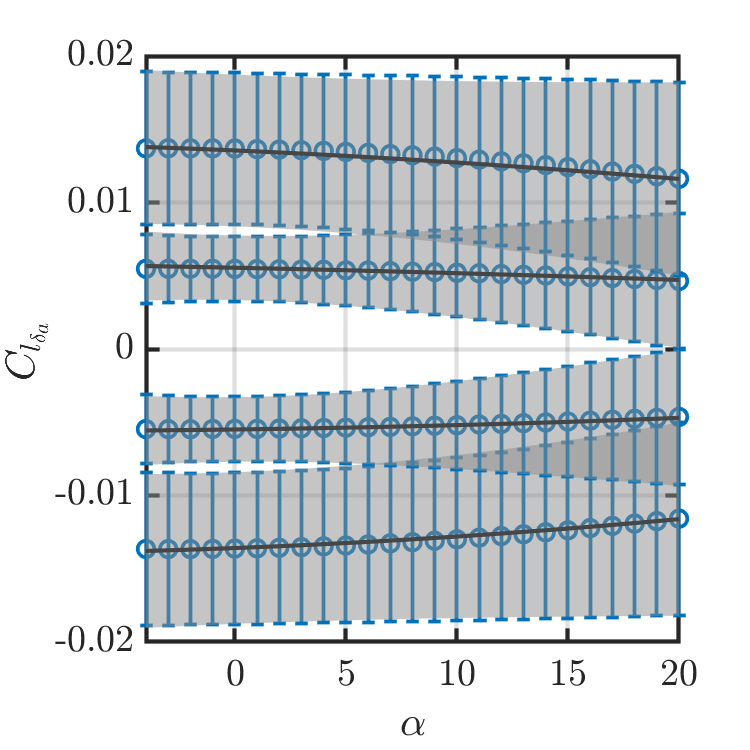
\includegraphics[trim=0 0 0 0, clip, width=.48\textwidth]{code/image_gen/gmatt/1f/avl/images/gps/CRMAIL_beta=4.png} 
    }
    \end{subfigure}
    \hfill
    \begin{subfigure}[\label{subfig:gtt_avl_ctrl_defl}Variation in $\delta_a$ at $\alpha = 8^\circ$ and $\beta=4^\circ$]{
        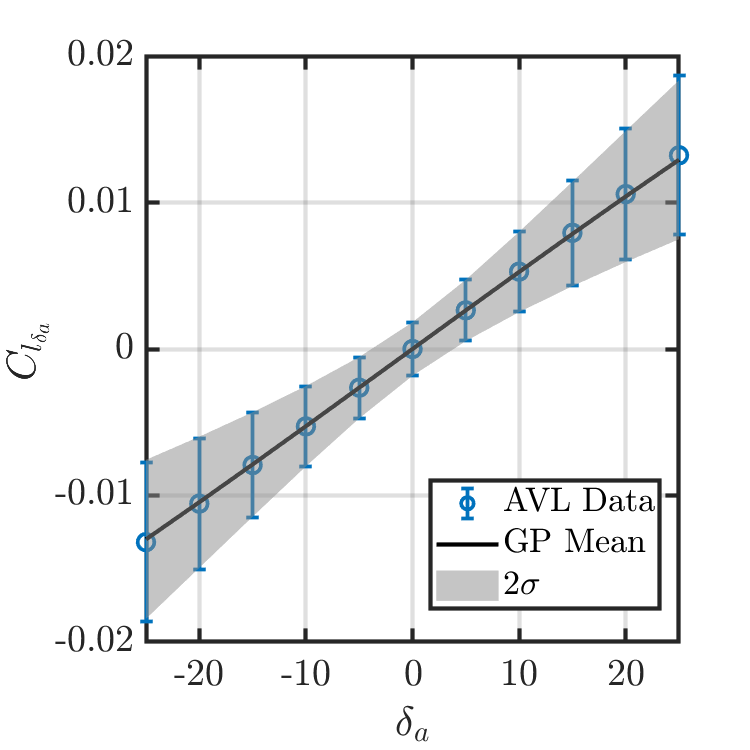
\includegraphics[trim=0 0 0 0, clip, width=.48\textwidth]{code/image_gen/gmatt/1f/avl/images/gps/CRMAIL_alpha=8_beta=4.png} 
    }
    \end{subfigure}
    \caption{Visualization of the 3-Dimensional AVL data and resulting single-fidelity GP for the rolling moment due to aileron deflections. \label{fig:gtt_avl_ctrl_gps}}
\end{figure}

\begin{figure}
    \centering
    \begin{subfigure}[\label{subfig:gtt_wt_ctrl_surf}3-Dimensional function in $\alpha$, $\beta$, and $\delta_a$] {
        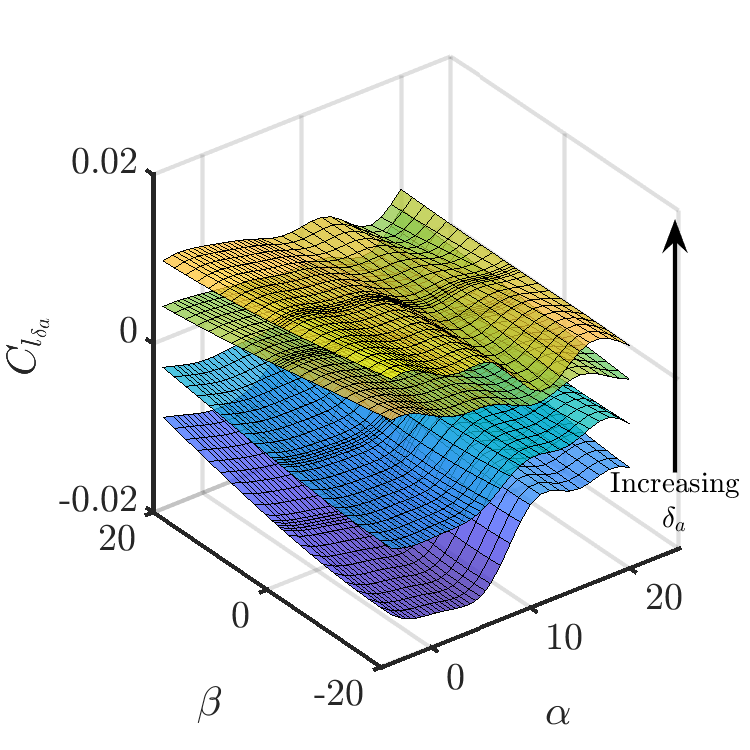
\includegraphics[trim=0 0 0 0, clip, width=.48\textwidth]{code/image_gen/gmatt/1f/wt/images/gps/CRMAIL.png} }
    \end{subfigure}
    \hfill
    \begin{subfigure}[\label{subfig:gtt_wt_ctrl_beta}Variation in $\beta$ at $\alpha=8^\circ$]{
        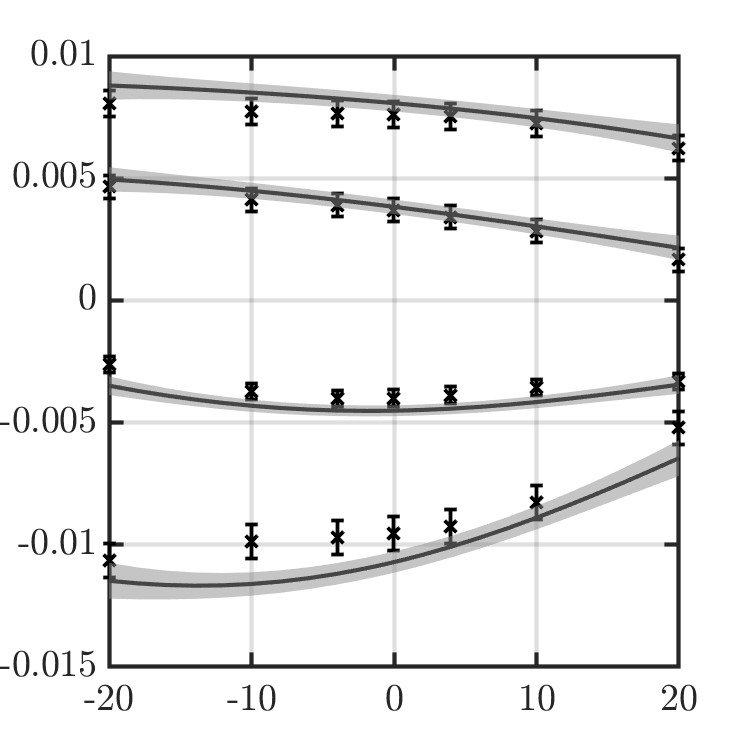
\includegraphics[trim=0 0 0 0, clip, width=.48\textwidth]{code/image_gen/gmatt/1f/wt/images/gps/CRMAIL_alpha=8.png}
    }
    \end{subfigure}
    \hfill
    \begin{subfigure}[\label{subfig:gtt_wt_ctrl_alpha}Variation in $\alpha$ at $\beta=4^\circ$]{
        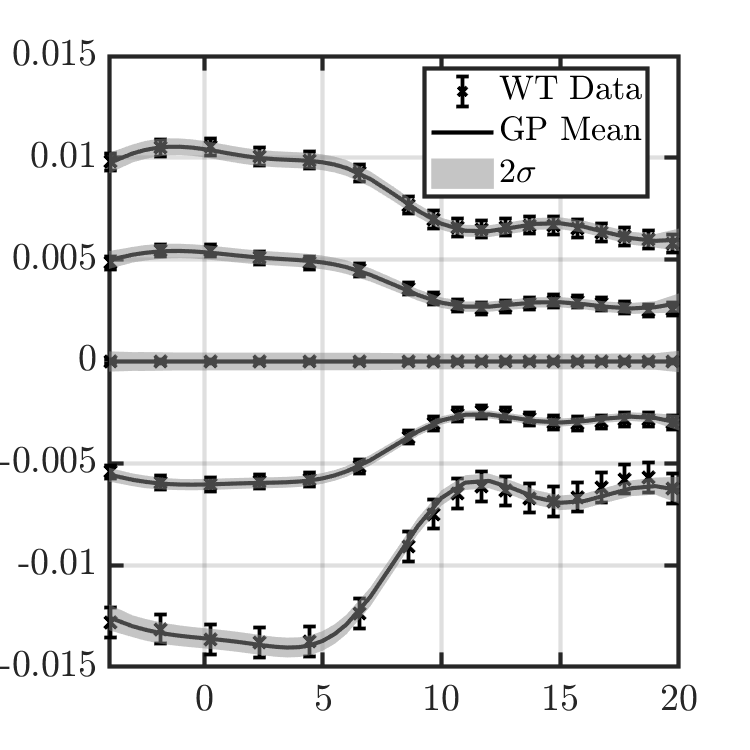
\includegraphics[trim=0 0 0 0, clip, width=.48\textwidth]{code/image_gen/gmatt/1f/wt/images/gps/CRMAIL_beta=4.png} 
    }
    \end{subfigure}
    \hfill
    \begin{subfigure}[\label{subfig:gtt_wt_ctrl_defl}Variation in $\delta_a$ at $\alpha = 8^\circ$ and $\beta=4^\circ$]{
        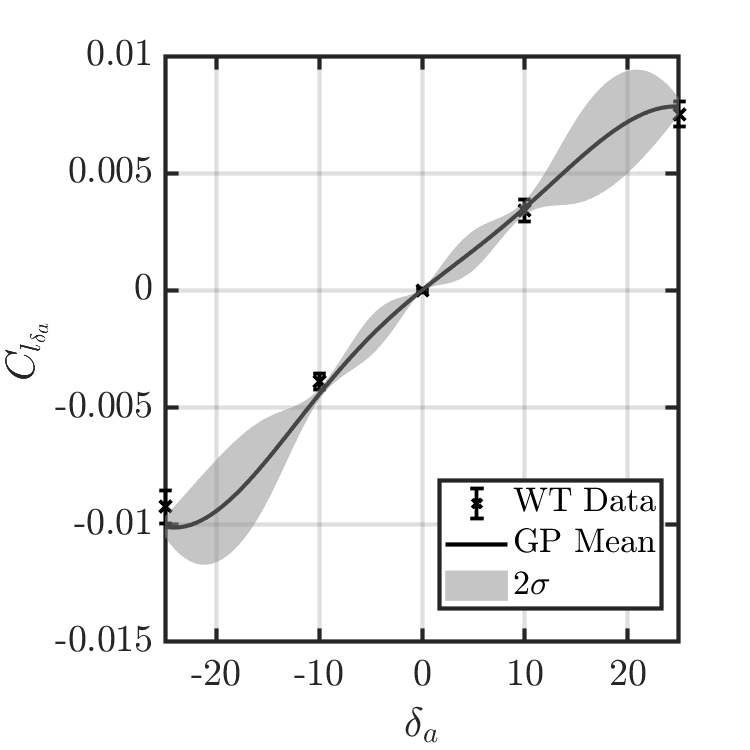
\includegraphics[trim=0 0 0 0, clip, width=.48\textwidth]{code/image_gen/gmatt/1f/wt_old/images/gps/CRMAIL_alpha=8_beta=4.png} 
    }
    \end{subfigure}
    \caption{Visualization of the 3-Dimensional WT data and resulting single-fidelity GP for the rolling moment due to aileron deflections. \label{fig:gtt_wt_ctrl_gps}}
\end{figure}

Figures \ref{subfig:gtt_avl_ctrl_surf} and \ref{subfig:gtt_wt_ctrl_surf} present stacks of surfaces where each surface represents $C_{l_{\delta_a}}$ as a function of $\alpha$ and $\beta$ at a particular aileron deflection angle ($\delta_a$).
Explicitly, the lowest surface in both figures corresponds to $\delta_a = -25^\circ$.
At the lowest level, the AVL data does capture the general trend of increasing $\delta_a$ leading to increased rolling moment, but there is a clear contrast in the linear trends learned from the AVL data and the non-linear trends represented in the wind tunnel data. 

In Figures \ref{subfig:gtt_avl_ctrl_beta} and \ref{subfig:gtt_wt_ctrl_beta}, the angle of attack is kept constant, $\alpha = 8^\circ$ and $C_{l_{\delta_a}}$ is represented as a function of $\beta$ at different values of $\delta_a$. 
For the AVL-based results (Figure \ref{subfig:gtt_avl_ctrl_beta}), blue circles and the associated error bars represent the uncertainty in the data.
The error bars are pretty large, and they result in overlapping of the gray $2\sigma$ uncertainty estimates at different $\delta_a$. 
For the WT-based results (Figure \ref{subfig:gtt_wt_ctrl_beta}), the uncertainty is a lot lower, but there is some discrepancy in the data points (black crosses) and the GP mean estimate (solid black line).
This discrepancy is not an error in the GP; instead, it is a consequence of the multi-dimensional hyper-parameters learned while maximizing the model's log-likelihood (Equation \ref{equ:hyp_param_sf}). 
Regularization prevents over-fitting of the data. 

For Figures \ref{subfig:gtt_avl_ctrl_alpha} and \ref{subfig:gtt_wt_ctrl_alpha}, the angle of slideslip is kept constant, $\beta=4^\circ$ and $C_{l_{\delta_a}}$ is represented as a function of $\alpha$ at different values of $\delta_a$.
There is a similar overlap of the uncertainty estimate for the AVL-based GP and a capturing of non-linear trends by the WT-based GP. 

Figures \ref{subfig:gtt_avl_ctrl_defl} and \ref{subfig:gtt_wt_ctrl_defl} present $C_{l_{\delta_a}}$ as a function of $\delta_a$ when $\alpha = 8^\circ$ and $\beta = 4^\circ$.
There is a distinctly linear relationship between the rolling moment and the aileron deflection. 
While the AVL-based GP respects the uncertainty in the data across the domain, the WT-based GP predicts increased uncertainty between data points. 
In these areas, the uncertainty in the model parameters is surpassing the uncertainty in the data.
This trend indicates the need for additional data between the current set of aileron deflection angles for which wind tunnel data is available.
Using the multi-fidelity framework addresses this need.

\subsection{Multi-fidelity Databases}
The lower-fidelity AVL data can augment the limited wind tunnel data points to create a better surrogate model.
Figure \ref{fig:gtt_2f_ctrl_gps} continues in the vein of the previous figures with stacks of lines and surfaces representing the rolling moment at different aileron deflection angles. 
When compared to the single-fidelity WT-based GP shown in Figure \ref{fig:gtt_wt_ctrl_gps}, the results are similar with the notable exception of Figure \ref{subfig:gtt_2f_ctrl_defl}.
When using the abundant AVL data to supplement the sparse WT data in the aileron deflection dimension, the ballooning of the uncertainty estimates between data points disappears. 
The uncertainty estimates across the domain are reduced without using any more high-fidelity data. 

\begin{figure}
    \centering
    \begin{subfigure}[\label{subfig:gtt_2f_ctrl_surf}3-Dimensional function in $\alpha$, $\beta$, and $\delta_a$] {
        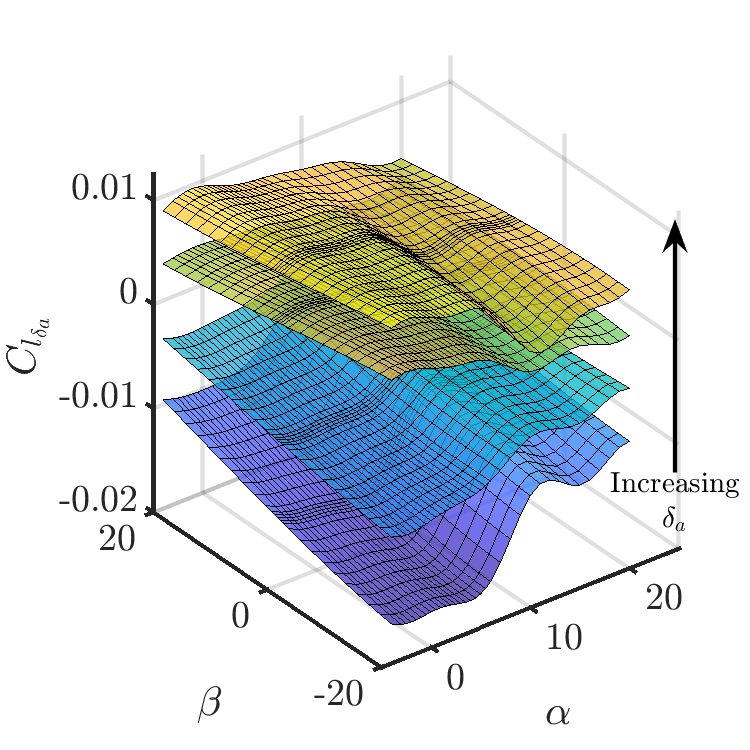
\includegraphics[trim=0 0 0 0, clip, width=.48\textwidth]{code/image_gen/gmatt/3f/images/gps/CRMAIL.png} }
    \end{subfigure}
    \hfill
    \begin{subfigure}[\label{subfig:gtt_2f_ctrl_beta}Variation in $\beta$ at $\alpha=8^\circ$]{
        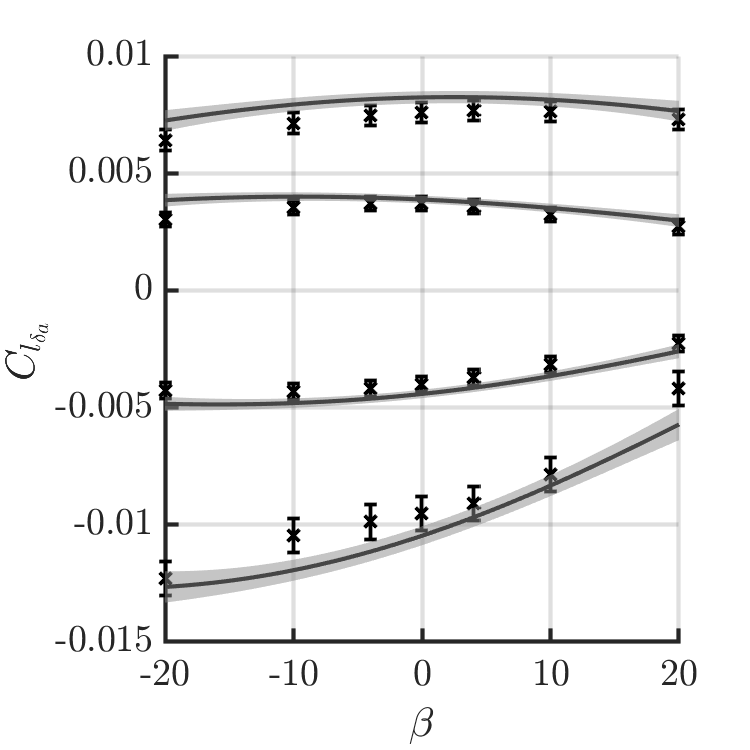
\includegraphics[trim=0 0 0 0, clip, width=.48\textwidth]{code/image_gen/gmatt/3f/images/gps/CRMAIL_alpha=8.png}
    }
    \end{subfigure}
    \hfill
    \begin{subfigure}[\label{subfig:gtt_2f_ctrl_alpha}Variation in $\alpha$ at $\beta=4^\circ$]{
        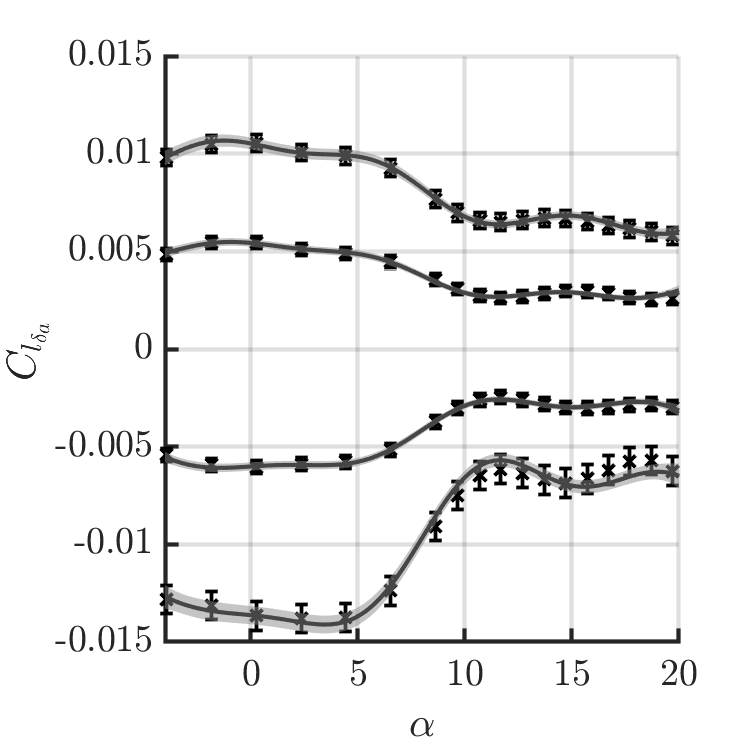
\includegraphics[trim=0 0 0 0, clip, width=.48\textwidth]{code/image_gen/gmatt/3f/images/gps/CRMAIL_beta=4.png} 
    }
    \end{subfigure}
    \hfill
    \begin{subfigure}[\label{subfig:gtt_2f_ctrl_defl}Variation in $\delta_a$ at $\alpha = 8^\circ$ and $\beta=4^\circ$]{
        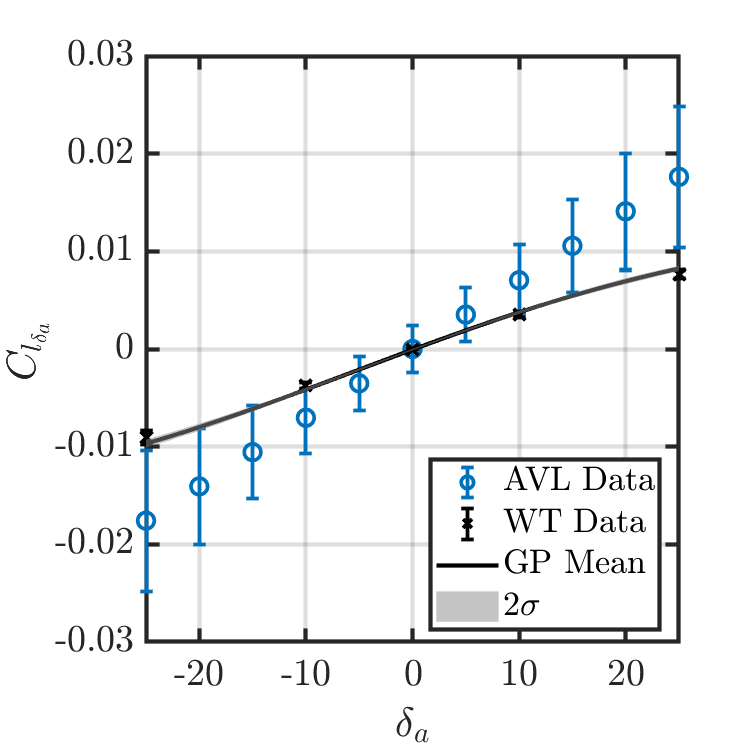
\includegraphics[trim=0 0 0 0, clip, width=.48\textwidth]{code/image_gen/gmatt/3f/images/gps/CRMAIL_alpha=8_beta=4.png} 
    }
    \end{subfigure}
    \caption{Visualization of the 3-Dimensional AVL and WT data, and the resulting two-fidelity GP for the rolling moment due to aileron deflections. \label{fig:gtt_2f_ctrl_gps}}
\end{figure}

This feature is a significant advantage of using multi-fidelity data, but there is a caveat.
The lower fidelity data needs to capture some relevant trends in the high-fidelity data. 
If the lower-fidelity trends contradict those seen in the high-fidelity data, then the low-fidelity data only corrupts the GP predictions. 
The multi-fidelity GP is trained on the difference between the low-fidelity data and the high-fidelity data. 
If there is no correlation between the low-fidelity and the high-fidelity data, then the difference between the two sets of data provides no useful information and only adds noise to the system. 
This issue, in turn, would prevent the multi-fidelity fit from performing as well or better than the single-fidelity fits. 

With the numerous multi-fidelity GP defining the aerodynamics and controls databases for the GTT aircraft created, flight simulations can be run using deterministic samples taken from these models.
These samples introduce minor variations in the aircraft's performance metrics that respect the GP error estimates resulting from the uncertainty in the underlying analysis data.


% --------------------------------------
% Certification by Analysis
% --------------------------------------
% \chapter{Certification by Analysis}

The increased reliance on simulation techniques for design analysis begs the question, can simulated analyses ever replace experimental ones?
Is it possible to complete parts of the flight certification process without first having to build a prototype of the aircraft and then putting it through flight testing?
This goal is of particular interest to the aerospace industry and is often referred to as Certification by Analysis (CbA).
To achieve this, simulation capabilities would have to be as accurate, if not more accurate, than what is possible with flight testing.  
There are many required improvements to simulation capabilities \cite{slotnick_cfd_nodate} that will take years to develop.

In the interim, quantifying the uncertainties in the analysis techniques allows us to rigorously handle current shortcomings and visualize their effect on flight performance predictions and, ultimately, predicted performance in flight testing.
While this will not be replacing real-world air-worthiness testing any time soon, it provides aircraft designers a method to estimate the likelihood that a design will pass or fail a certification test. 

The current aircraft design would have certain performance characteristics associated with it which can be represented as probabilistic aerodynamics and controls databases using multi-fidelity GP regression introduced in \ref{chap:mf_gp}.
These databases can be stochastically sampled to create multiple representations of the same aircraft that vary slightly in their performance.
The slight variations arise out of, and respect, the uncertainties in the analysis techniques used. 
Flight simulation software is used to run each of these aircraft samples through a certification maneuver of interest.
The results of the numerous simulations can be post-processed to calculate what percentage of the aircraft samples passed or failed the certification test.
This provides a quantifiable metric for the probability that the aircraft design, as it is best understood at that time, will succeed in the air-worthiness test.

In addition to a probability of success/failure, by looking at the variation in the flight characteristics of the different samples, this framework also provides data on how current uncertainties in performance predictions affect test results.
Based to these results, the design might need to be changed to ensure a better success rate, or higher-fidelity analysis methods with less uncertainty might need to be used to reduce the spread in the flight characteristics. 
These are direct benefits of the early handling of uncertainties in the design process to preempt possible issues in the future. 

This chapter presents the first steps in creating a rigorous methodology for CbA.
Contributions made in uncertainty quantification (Chapter \ref{chap:rans_uq}), multi-fidelity modeling (Chapter \ref{chap:mf_gp}), and probabilistic aerodynamics and controls databases (Chapter \ref{chap:aero_db}) are combined to create this framework.
Section \ref{sec:maneuver} presents a flight certification maneuver of interest that is taken directly from the official flight testing guide used by the Federal Aviation Administration (FAA) \cite{romanowski_flight_2018}.
Section \ref{sec:sim_procedure} detail the use of probabilistic aerodynamics and controls databases to simulate the maneuver of interest.
Finally, Section \ref{sec:cba_results} presents the results of performing the virtual flight testing and compares the use of different fidelity levels, and amounts of data. 
 fa
 

\section{Maneuver of Interest} \label{sec:maneuver}

A certification maneuver is needed to demonstrate CbA.
The Generic T-tail Transport, as the name suggests, is based on a commercial transport class aircraft.
It is most closely related to the Bombardier CRJ 700.
A few guiding principles were used in selecting the maneuver of interest:
\begin{itemize}
    \item Real-world certification requirement that the aircraft would be required to pass.
    \item Availability of data required to simulate the maneuver adequately.
    \item Preferably a lateral or directional maneuver that can leverage the multi-dimensional experimental data.
    \item Emphasis on control input to utilize control derivative data.
    \item A quantifiable metric to determine success or failure of the certification maneuver.
\end{itemize}

Based on these guidelines and with the help of industry experts at The Boeing Company, a maneuver was picked from the FAA's \textit{Flight Test Guide for Certification of Transport Category Airplanes} \cite{romanowski_flight_2018}.
Within Chapter \textit{5.3 Directional and Lateral Control} of the guide, the \textit{Lateral Control: Roll Capability \S 25.147(d)} maneuver was chosen.   
The testing procedure is paraphrased as: 
\begin{enumerate}
    \item Airplane starts in a trimmed state for steady straight flight at maximum takeoff speed.
    \item Establish a steady $30^\circ$ banked turn.
    \item Roll the airplane to a $30^\circ$ bank angle in the other direction.
    \item Aircraft must have sufficient roll authority to perform the $60^\circ$ change in bank angle in no more than $11$ seconds. 
    \item The aircraft must be able to do this with one engine inoperative, specifically the one that makes this maneuver more difficult.

\end{enumerate}

Two additional parameters mentioned in the guide relate to the maneuver being unchecked: the roll maneuver does not need to stop immediately after achieving the $30 ^\circ$ bank angle, and the aircraft should avoid excessive sideslip and bank angle during recovery.
Since these are not easily quantifiable parameters, they are not explicitly enforced in the flight simulation.
Regarding the airplane flap configuration, the guide specifies \textit{"Wing flaps in the most critical takeoff position."}
This statement is vague, and while some simulations deployed the flaps at $15^\circ$ per the CRJ700 Pilot's Handbook, most simulation results presented do not use flap deflections. 
It was infeasible to run RANS CFD simulations with flaps deployed due to the absence of an accurate geometry with deployed flaps and the significant increase in computational cost that it would merit.  
While engine data is not readily available and, consequently, some modeling was required, the maneuver satisfies all the guiding principles and provides an excellent platform to showcase the culmination of all the different parts of the work.

Figure \ref{fig:roll_maneuver} shows a visual representation of the maneuver. 
For this image, the positive x-axis and the airplane's nose are pointing out of the page.
For an aircraft that rolls from $\phi = +30^\circ$ to $-30^\circ$, having an inoperative right engine is the more difficult maneuver.
This difficulty arises from the thrust of the left engine inducing a yaw moment and, consequently, a roll moment that resists the roll maneuver.
Accordingly, the right engine is labeled as inoperative with the "x" over it.

\begin{figure}
    \center
    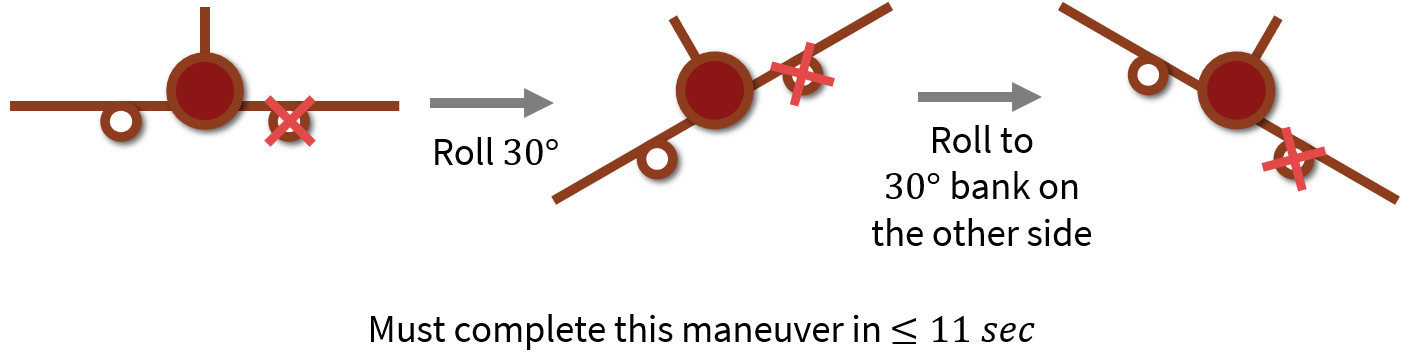
\includegraphics[width=0.95\textwidth]{suthesis/images/roll_maneuver.png}
    \caption{Graphical representation of Roll Capability certification maneuver. \label{fig:roll_maneuver}}
\end{figure}

\section{Simulation Procedure} \label{sec:sim_procedure}

Now that a flight certification maneuver has been chosen, a method to run a current aircraft design thorough the maneuver-of-interest needs to be be developed.
The aircraft design is represented using probabilistic multi-fidelity aerodynamics and controls databases as shown in \ref{sec:gtt_dbs}.
The uncertainty in the data that informs the databases, manifests itself in slight variations in the samples of the databases.
Each sample aerodynamic database has information about the forces and moments on an aircraft at various points in the flight envelope.
The controls database samples contain information about the moments induced on the aircraft due to various control surface deflections. 
These samples are run through flight simulation software that can integrate the force and moment information, combine it with the effects of control inputs, and perform a time-accurate maneuver that is defined in the simulation software. 

This part of the work leans heavily on the expertise of the The Boeing Company in flight simulation and control law mixing.
Due to proprietary and patent restrictions, exact implementation of the flight simulation code is unavailable but enough information is provided to outline the simulations' overarching methodology and workflow.

Figure \ref{fig:cfr147d_inputs} represents the steps required to simulate the airworthiness test. 
The first step in the simulation process is to convert the maneuver of interest, in this case the \textit{Lateral Control: Roll Capability \S 25.147(d)} maneuver, into a trajectory for the aircraft to follow. 
This maneuver is mostly defined by roll angle of the aircraft and is shown in Figure \ref{subfig:roll_angle}.
There are other parameters included in the trajectory definition, for example constant altitude to ensure a steady level turn, but the roll angle is of primary concern and is focused on here. 
The aircraft starts with steady level flight, rolls to an angle $\psi = +30^\circ$, and then completes the roll maneuver from $\psi = +30^\circ$ to $=-30^\circ$ in 11 seconds, as required by the certification maneuver. 

The required trajectory and 

\begin{figure}
    \centering
    \begin{subfigure}[Flight simulation trajectory definition for the roll angle of the aircraft. Derived from the air-worthiness test.] {
        \includegraphics[trim=0 0 0 0, clip, width=.55\textwidth]{suthesis/images/cfr147d_roll_angle.png}
        \label{subfig:roll_angle}
    }
    \end{subfigure}
    \hfill
    \begin{subfigure}[Roll acceleration that would be required for the aircraft to follow the roll angle trajectory]{
        \includegraphics[trim=0 0 0 0, clip, width=.55\textwidth]{suthesis/images/cfr147d_roll_acc.png} 
        \label{subfig:roll_acc}
    } 
    \end{subfigure}
    \hfill
    \begin{subfigure}[Left and right aileron deflections commanded to create the requisite roll accelerations]{
        \includegraphics[trim=0 0 0 0, clip, width=.55\textwidth]{suthesis/images/cfr147d_ail_defl.png} 
        \label{subfig:ail_defl}
    } 
    \end{subfigure}
    \caption{Steps required to convert the air-worthiness test into a the required inputs for the flight simulation of the maneuver. \label{fig:cfr147d_inputs}}
\end{figure}

\section{Monte-Carlo Analysis} \label{sec:mc_analysis}

The goal of 

\section{Results} \label{sec:cba_results}
With the aircraft maneuver and flight simulation process defined, results from running the GTT aircraft through the flight certification maneuver are discussed in this section.
There are two over-arching goals of this work: first, to provide a framework that brings flight testing earlier in the aircraft design process, and second, to create the most accurate flight simulation results while minimizing the cost of the underlying analyses. 
To this end, this section first focuses on comparing simulations that are run using purely high-fidelity experimental data, to those run using low-fidelity and multi-fidelity data that would be available early in the design process.
Then the cost-reduction aspect is explored by harnessing the benefits of multi-fidelity databases that use small subsets of the high-fidelity data. 
For all the results in this section, simulations are conducted with the right engine inoperative, and all modifications discussed in Section \ref{subsec:sim_mods} are applied.

utilize multi-fidelity GP models that are created using various combinations of low-fidelity AVL data, medium-fidelity CFD simulation data, and high-fidelity experimental wind tunnel data, to those that utilize single-fidelity GP models created using purely high-fidelity data. 

\subsection{Simulations using Single- vs. Multi-Fidelity Databases} \label{subsec:sf_vs_mf_cba}




% --------------------------------------
% Conclusions
% --------------------------------------
% \chapter{Conclusions} \label{sec:conclusions}

In this paper, two main contributions have been presented in the context of multi-fidelity UQ applications of interest to the aerospace engineering industry, and to the simulation-based engineering community: a method to quantify model-form uncertainties in RANS CFD simulations, and a multi-fidelity Gaussian Process framework that combines data sources of varying accuracy to provide better estimates of QoIs and their uncertainties. Both of these methodologies were showcased using a real-world probabilistic aerodynamic database for a full-configuration aircraft, the NASA Common Research Model. 

The RANS UQ methodology uses eigenspace perturbations of the modeled Reynolds' stress tensor to create flow fields that push against the physical realizability constraints of the stress tensor. This methodology provided interval estimates on the QoIs based on the model-form uncertainties associated with turbulence modeling. Simulations at low angles of attack, where the turbulence model is able to accurately capture flow features, had smaller bounds than those performed at high angles of attack, where flow separation is significant and the turbulence model is unable to provide accurate predictions. The predicted bounds did not encapsulate the experimental data due to well known geometric discrepancies between the wind tunnel model and the model used for numerical simulations that resulted from unaccounted aeroelastic twist.

Previous work in multi-fidelity Gaussian processes was advanced by introducing noise in the observations of the QoIs. The RANS CFD simulations and associated uncertainty predictions were combined with low-fidelity data from AVL simulations, and high-fidelity data from wind tunnel experiments to create multi-fidelity surrogate models for $C_L$, $C_D$, and $C_m$ for the NASA CRM. These multi-fidelity fits were more accurate than single-fidelity GP fits on just the high-fidelity data at a significantly lower cost, showing that lower-fidelity data that is well correlated with higher-fidelity data can serve to augment high-fidelity data to improve predictive capabilities.  This is especially true in multi-dimensional operating spaces where the quantity of interest would require the use of a prohibitive number of high-fidelity simulations or wind-tunnel data points.

Finally, we would like the current work to serve as an early (and, necessarily, incomplete) example of the direction of evolution that would be beneficial for future engineering simulations. As industry increases its reliance on numerical simulations for design and analysis, it is essential to understand and address the shortcomings of such simulations. Quantifying uncertainties introduced by these predictive methodologies is the first step in extending their value. It enables the use of a reliability-based design process instead of the traditional, deterministic design methodology that makes no allowance for modeling uncertainties. Additionally, combining predictions from all the analysis methods that are used in the design process improves their predictive capability with lower computational cost. 



\appendix
\chapter{A Long Proof}
...
\bibliographystyle{plain}
\bibliography{References}
\end{document}
